\documentclass[12pt]{article}
\usepackage[margin=2.5cm]{geometry}
\usepackage{enumerate}
\usepackage{amsfonts}
\usepackage{amsmath}
\usepackage{fancyhdr}
\usepackage{amsmath}
\usepackage{amssymb}
\usepackage{amsthm}
\usepackage{mdframed}
\usepackage{graphicx}
\usepackage{subcaption}
\usepackage{adjustbox}
\usepackage{listings}
\usepackage{xcolor}
\usepackage{booktabs}
\usepackage[utf]{kotex}
\usepackage{hyperref}
\usepackage{accents}

\definecolor{codegreen}{rgb}{0,0.6,0}
\definecolor{codegray}{rgb}{0.5,0.5,0.5}
\definecolor{codepurple}{rgb}{0.58,0,0.82}
\definecolor{backcolour}{rgb}{0.95,0.95,0.92}

\lstdefinestyle{mystyle}{
    backgroundcolor=\color{backcolour},
    commentstyle=\color{codegreen},
    keywordstyle=\color{magenta},
    numberstyle=\tiny\color{codegray},
    stringstyle=\color{codepurple},
    basicstyle=\ttfamily\footnotesize,
    breakatwhitespace=false,
    breaklines=true,
    captionpos=b,
    keepspaces=true,
    numbers=left,
    numbersep=5pt,
    showspaces=false,
    showstringspaces=false,
    showtabs=false,
    tabsize=1
}

\lstset{style=mystyle}

\pagestyle{fancy}
\renewcommand{\headrulewidth}{0.4pt}
\lhead{CSC 343}
\rhead{Worksheet 15 Solution (Final)}

\begin{document}
\title{CSC343 Worksheet 15 Solution (Final)}
\maketitle

\begin{enumerate}[1.]
    \item

    \begin{itemize}
        \item E/R Diagram

        \begin{center}
        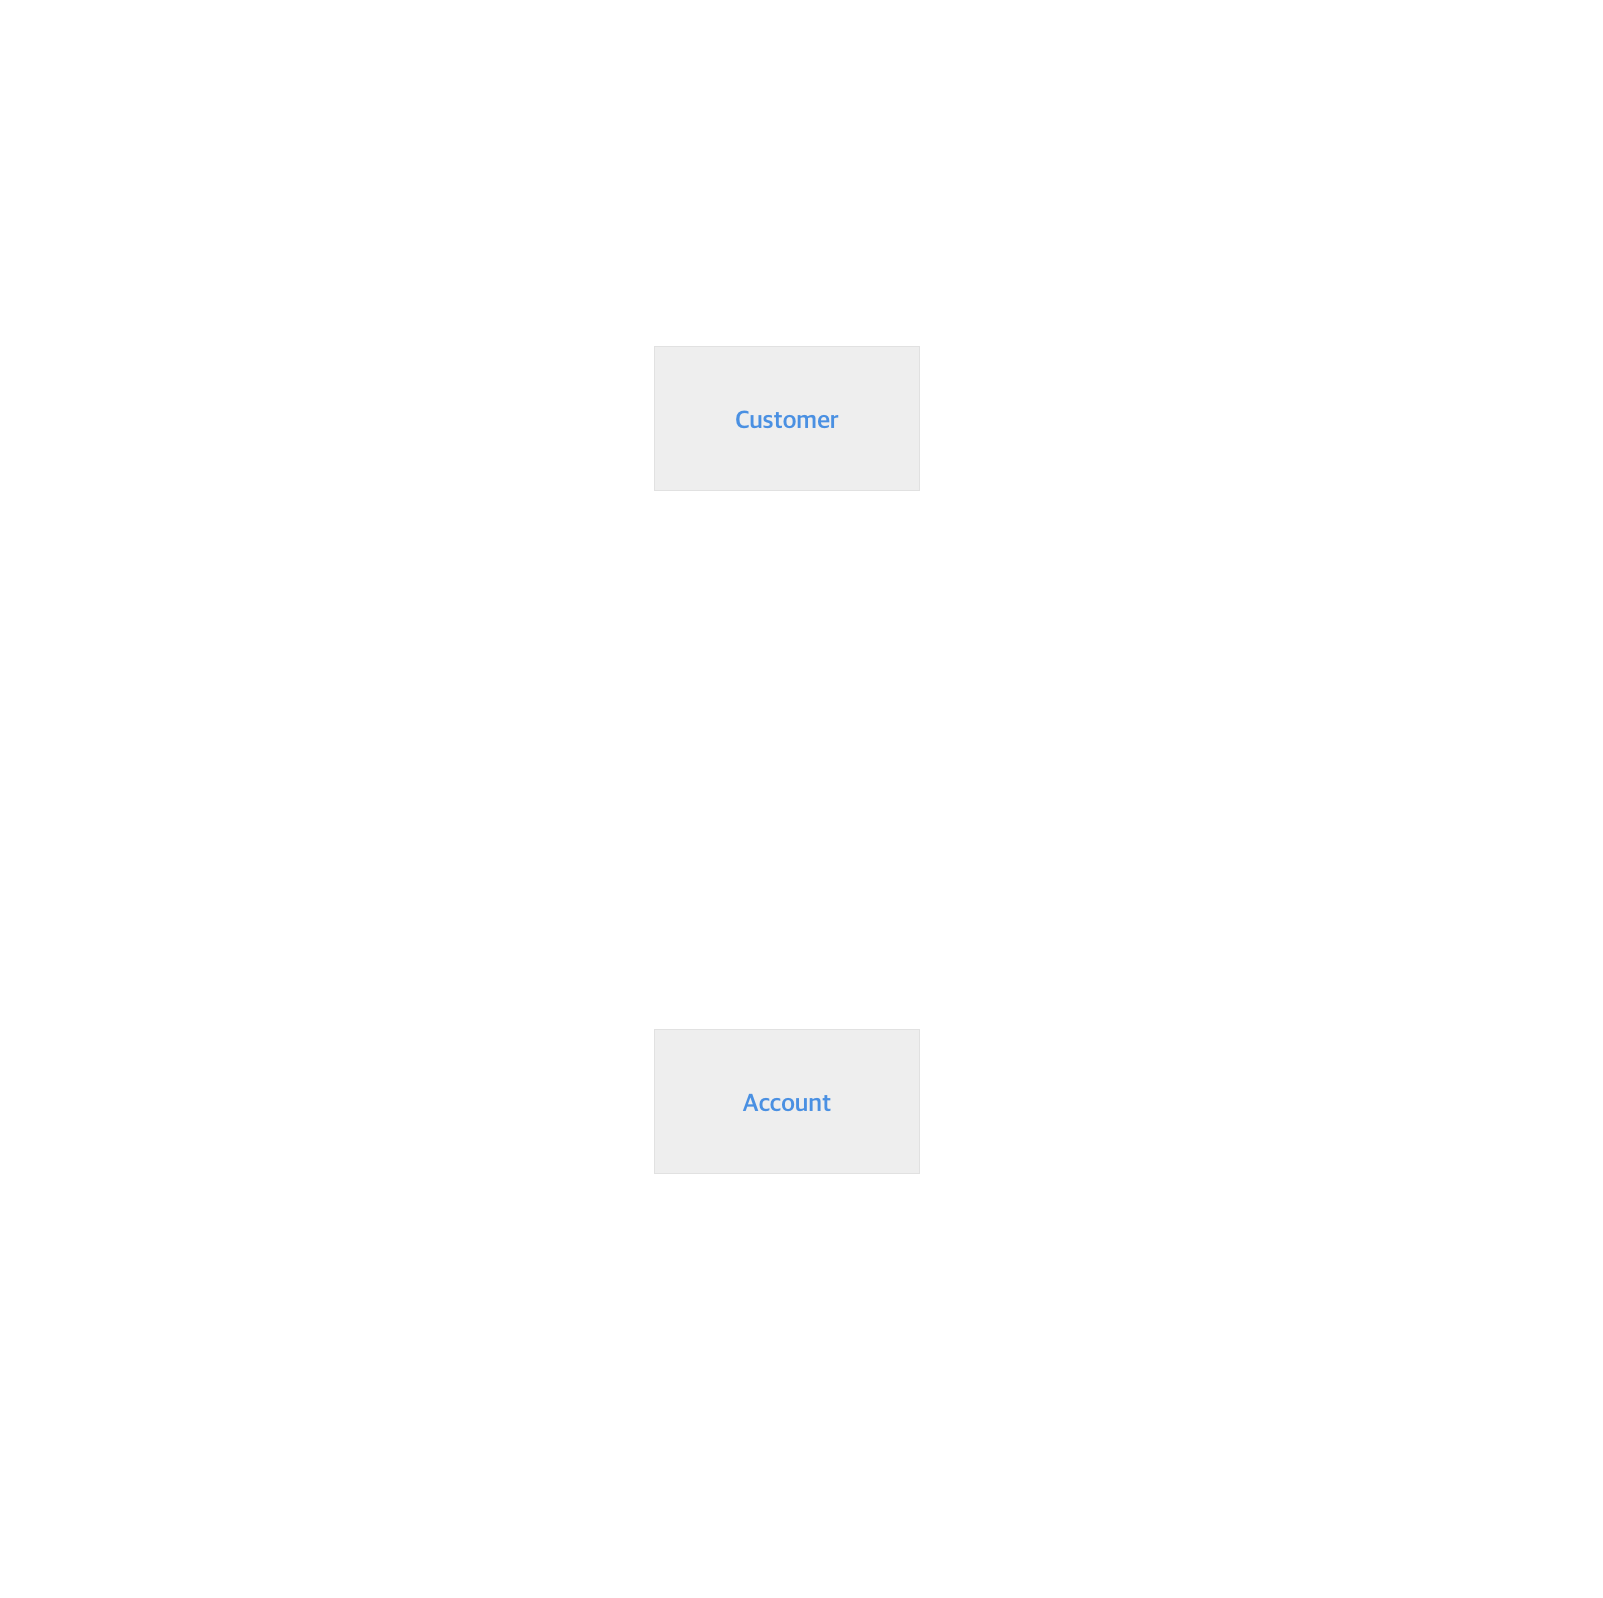
\includegraphics[width=0.7\linewidth]{images/worksheet_15_solution_9.png}
        \end{center}

        \item UML

        \begin{center}
        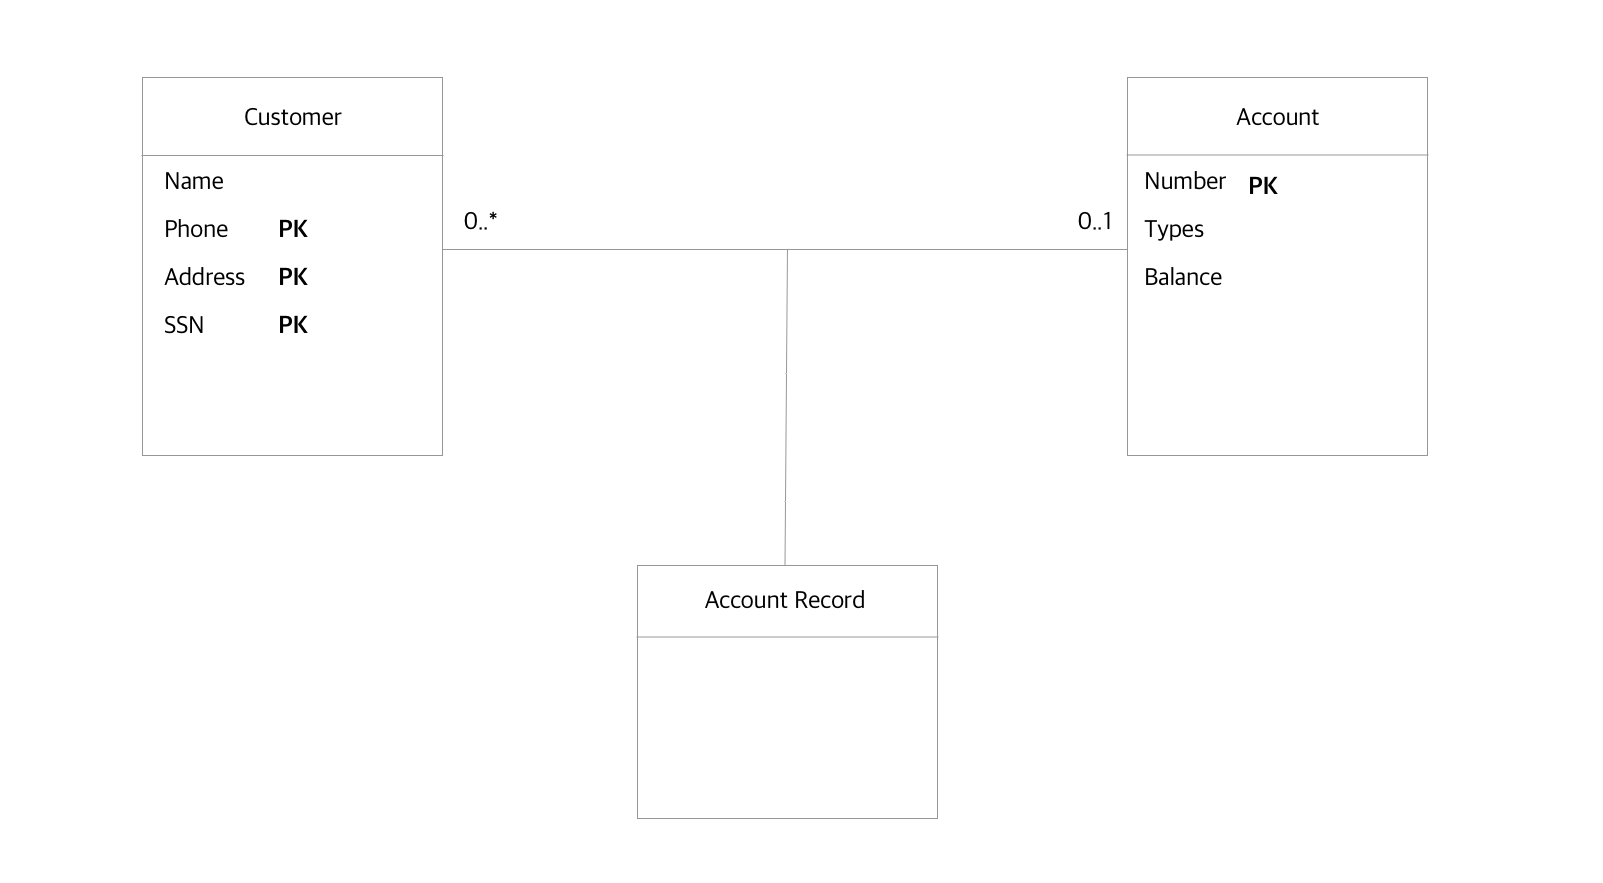
\includegraphics[width=\linewidth]{images/worksheet_15_solution_10.png}
        \end{center}


    \end{itemize}

    \bigskip

    \underline{\textbf{Notes:}}

    \bigskip

    \begin{itemize}
        \item UML
        \begin{itemize}
            \item Was developed originally as a graphical notation for describing software designs in an object-oriented style
            \item Offers the same as E/R model, with the exception of multiway relationship
        \end{itemize}

        \begin{center}
        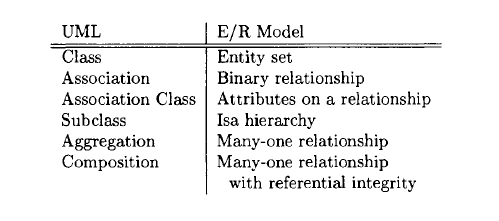
\includegraphics[width=0.7\linewidth]{images/worksheet_15_solution_1.png}
        \end{center}

        \item UML Class

        \begin{center}
        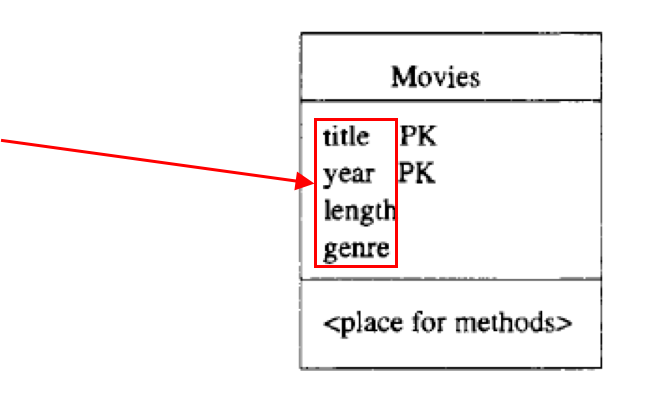
\includegraphics[width=0.5\linewidth]{images/worksheet_15_solution_2.png}
        \end{center}

        \item Associations

        \begin{center}
        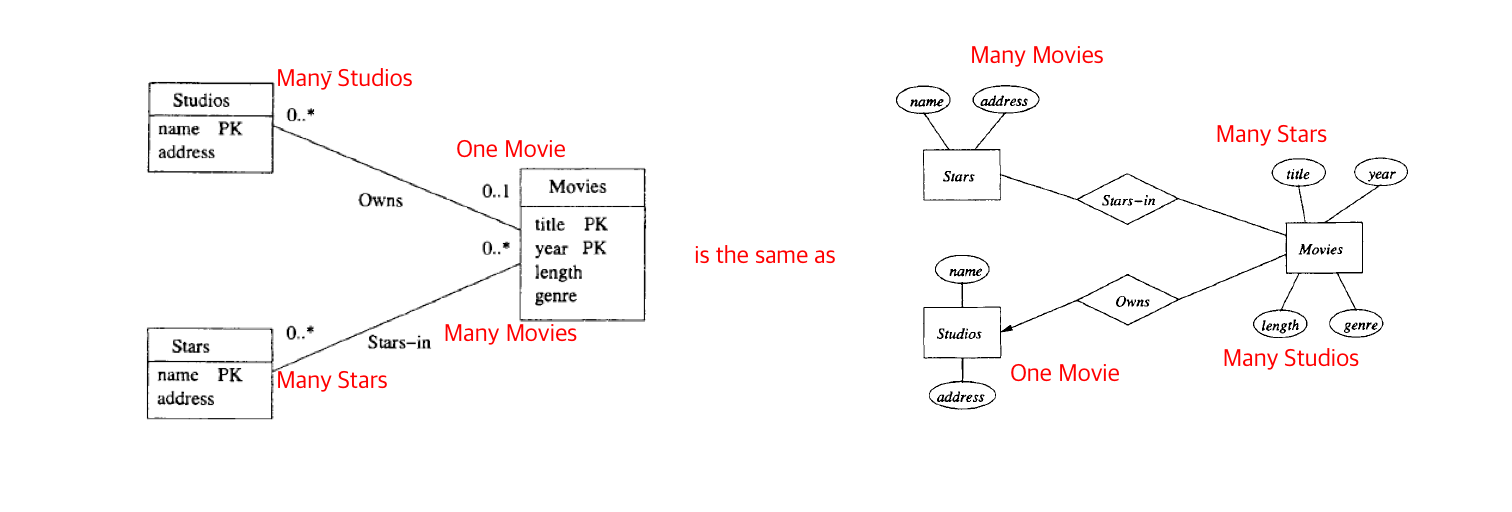
\includegraphics[width=\linewidth]{images/worksheet_15_solution_4.png}
        \end{center}

        \bigskip

        \underline{Multiplicity in UML}

        \bigskip

        \begin{center}
            \begin{tabular}{|c|c|c|}
                \hline
                Multiplicity & Option & Cardinality\\
                \hline
                0..0 & 0 & Collection must be empty\\
                \hline
                0..1 & & No instances or one instance\\
                \hline
                1..1 & 1 & Exactly one instance\\
                \hline
                0..* & * & Zero or more instance\\
                \hline
                5..5 & 5 & Exactly 5 instances\\
                \hline
                $m..n$ & & At least $m$ but no more than $n$ instances\\
                \hline
            \end{tabular}
        \end{center}

        \bigskip

        \underline{Example:}

        \begin{center}
        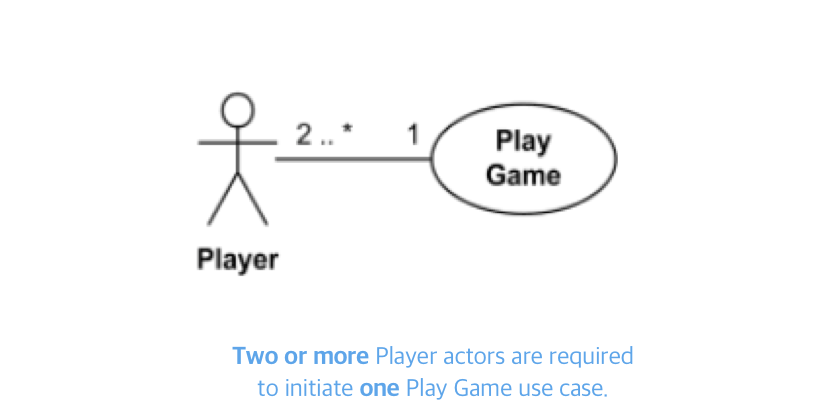
\includegraphics[width=0.7\linewidth]{images/worksheet_15_solution_3.png}
        \end{center}

        \bigskip

        \underline{References:}

        \bigskip

        \begin{enumerate}[1)]
            \item uml-diagrams, UML Multiplicity and Collections, \href{https://www.uml-diagrams.org/multiplicity.html}{link}
        \end{enumerate}

        \item Referential Integrity
        \begin{itemize}
            \item Means that a value appearing in one context must also appear in another
        \end{itemize}

        \bigskip

        \begin{center}
        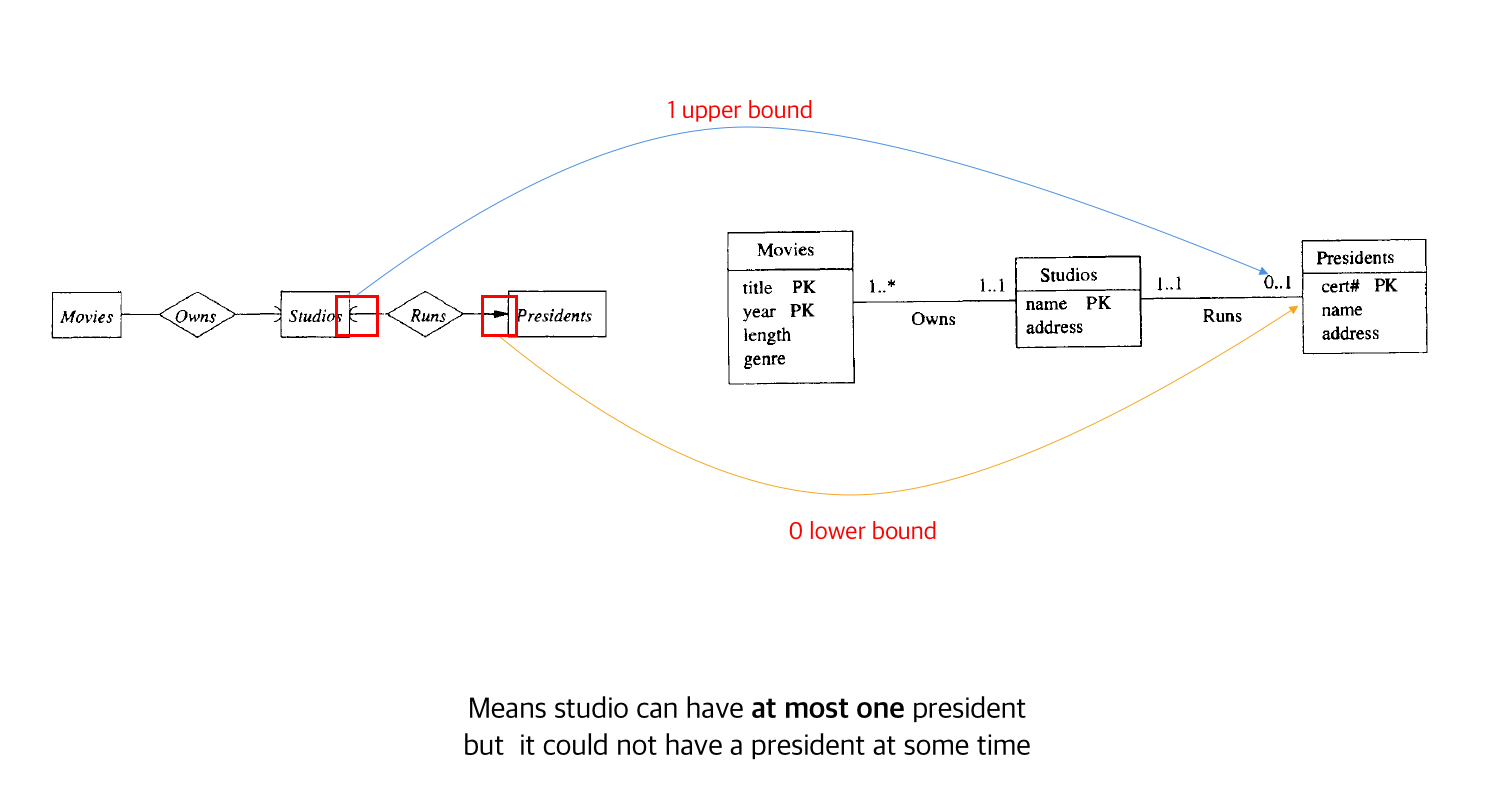
\includegraphics[width=\linewidth]{images/worksheet_15_solution_5.png}
        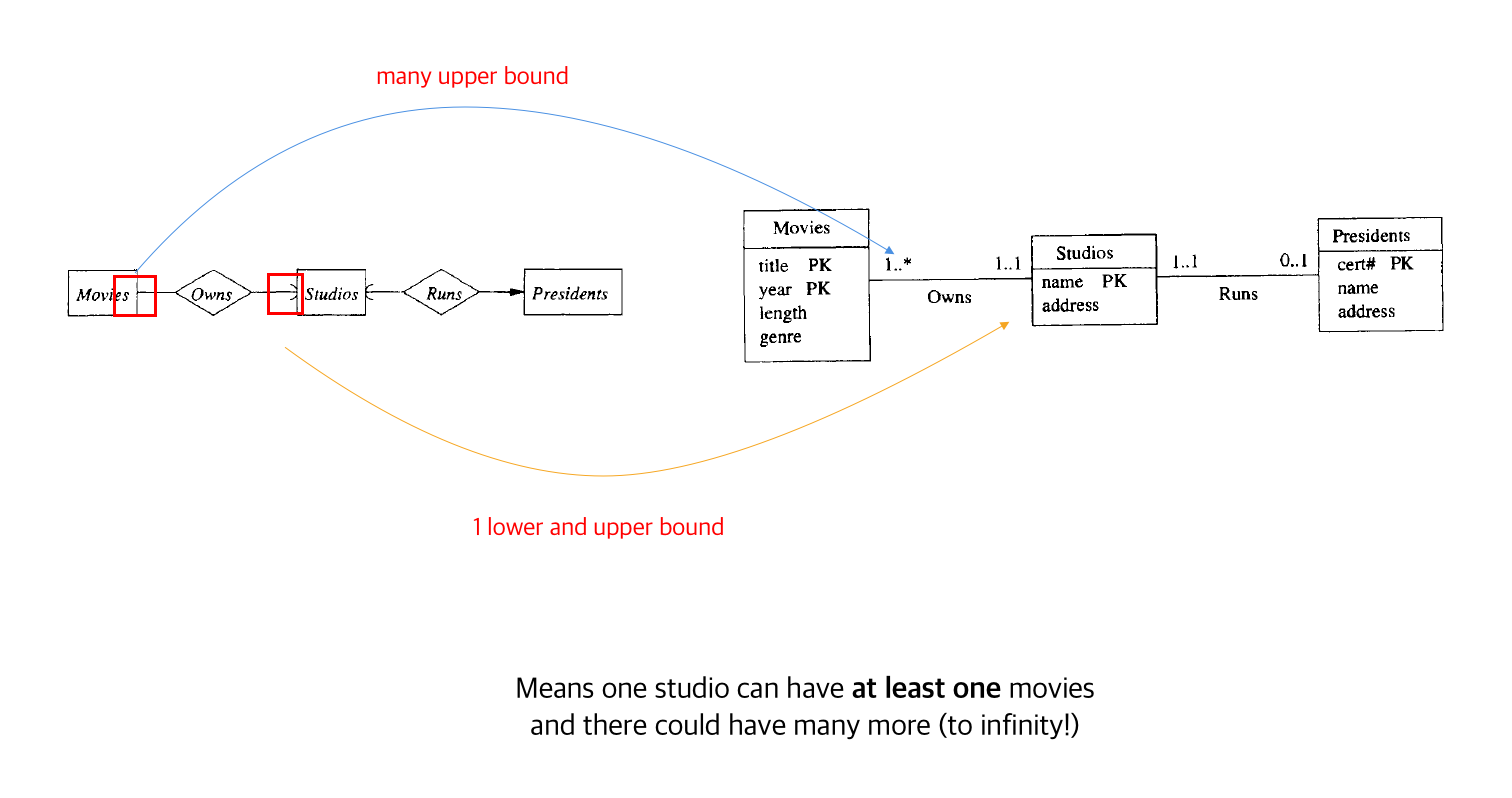
\includegraphics[width=\linewidth]{images/worksheet_15_solution_6.png}
        \end{center}

        \item Self-Assoiations

        \begin{center}
        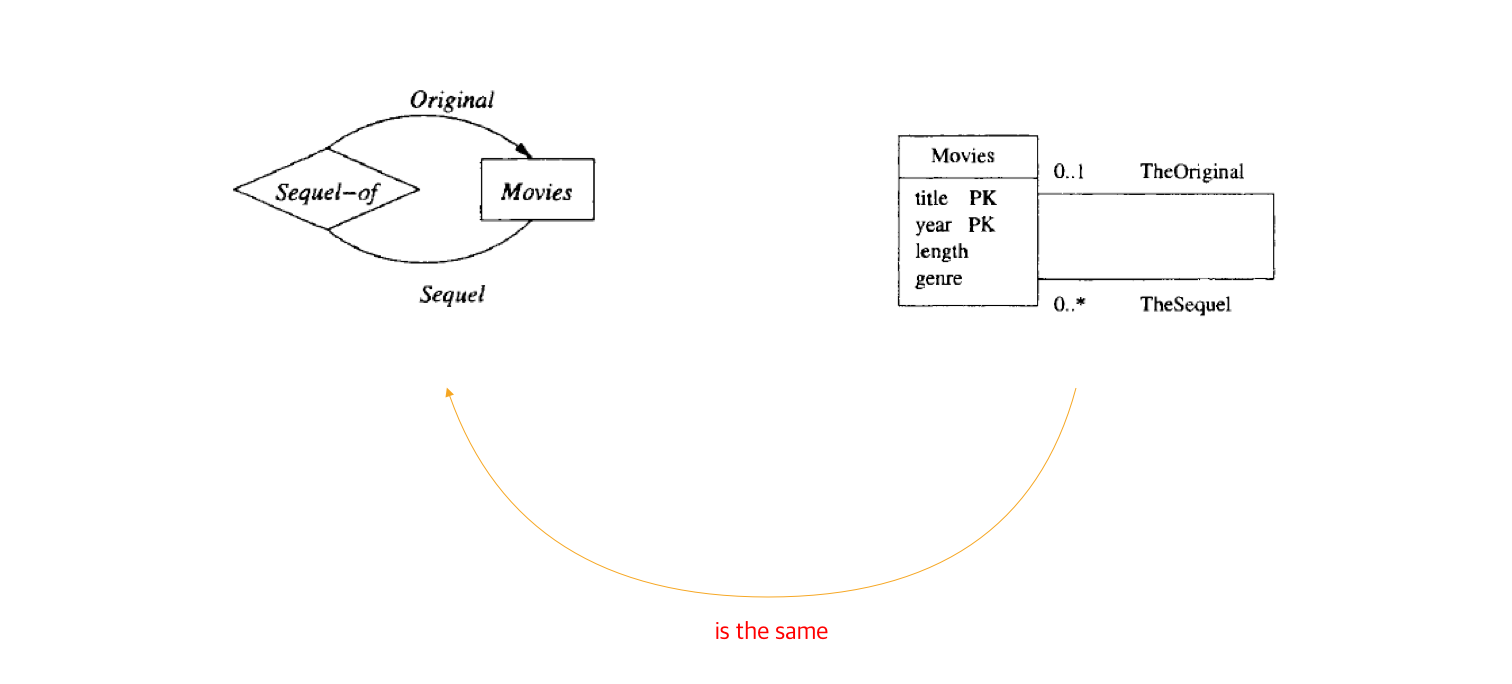
\includegraphics[width=\linewidth]{images/worksheet_15_solution_7.png}
        \end{center}


        \item Assoiations

        \begin{center}
        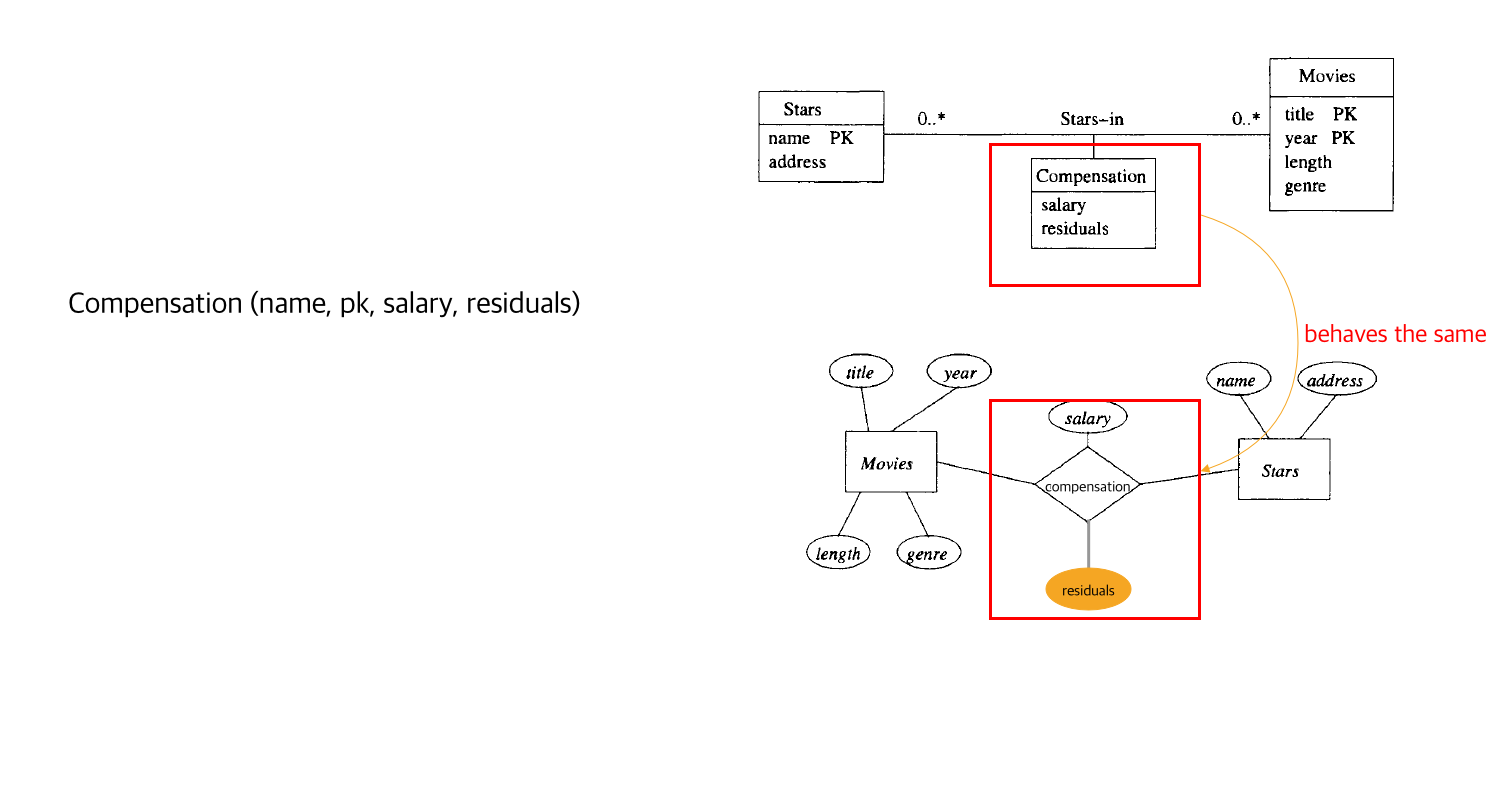
\includegraphics[width=\linewidth]{images/worksheet_15_solution_8.png}
        \end{center}

    \end{itemize}

    \item

    \begin{enumerate}[a)]
        \item

        \underline{\textbf{Solution:}}

        \begin{center}
        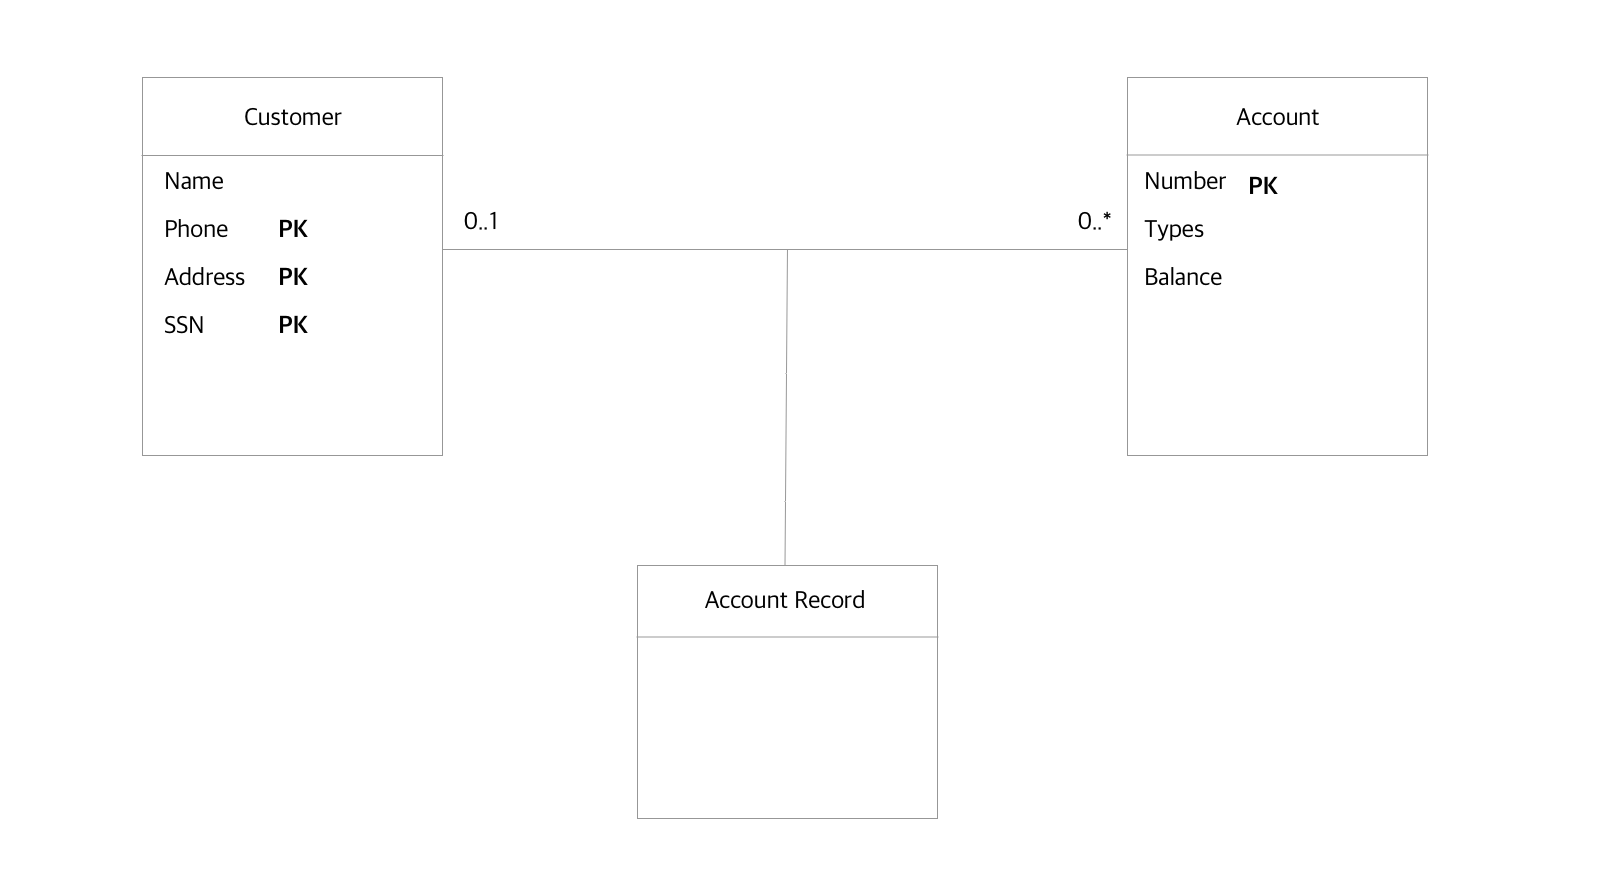
\includegraphics[width=\linewidth]{images/worksheet_15_solution_11.png}
        \end{center}

        \item

        \underline{\textbf{Solution:}}

        \begin{center}
        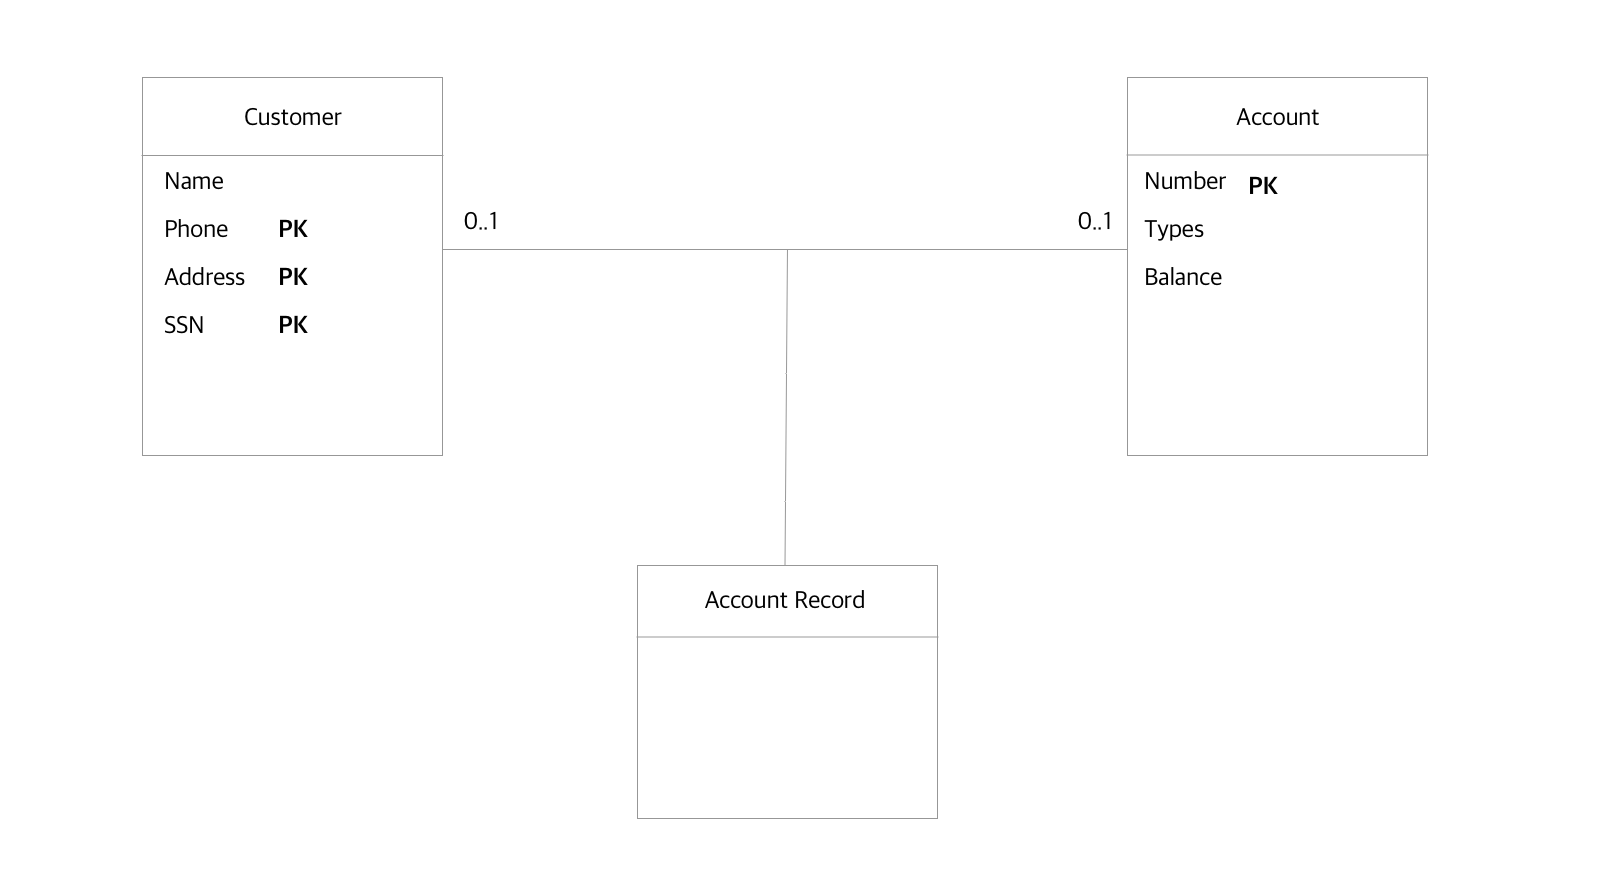
\includegraphics[width=\linewidth]{images/worksheet_15_solution_12.png}
        \end{center}
    \end{enumerate}

    \item

    \begin{itemize}
        \item E/R Diagram

        \begin{center}
        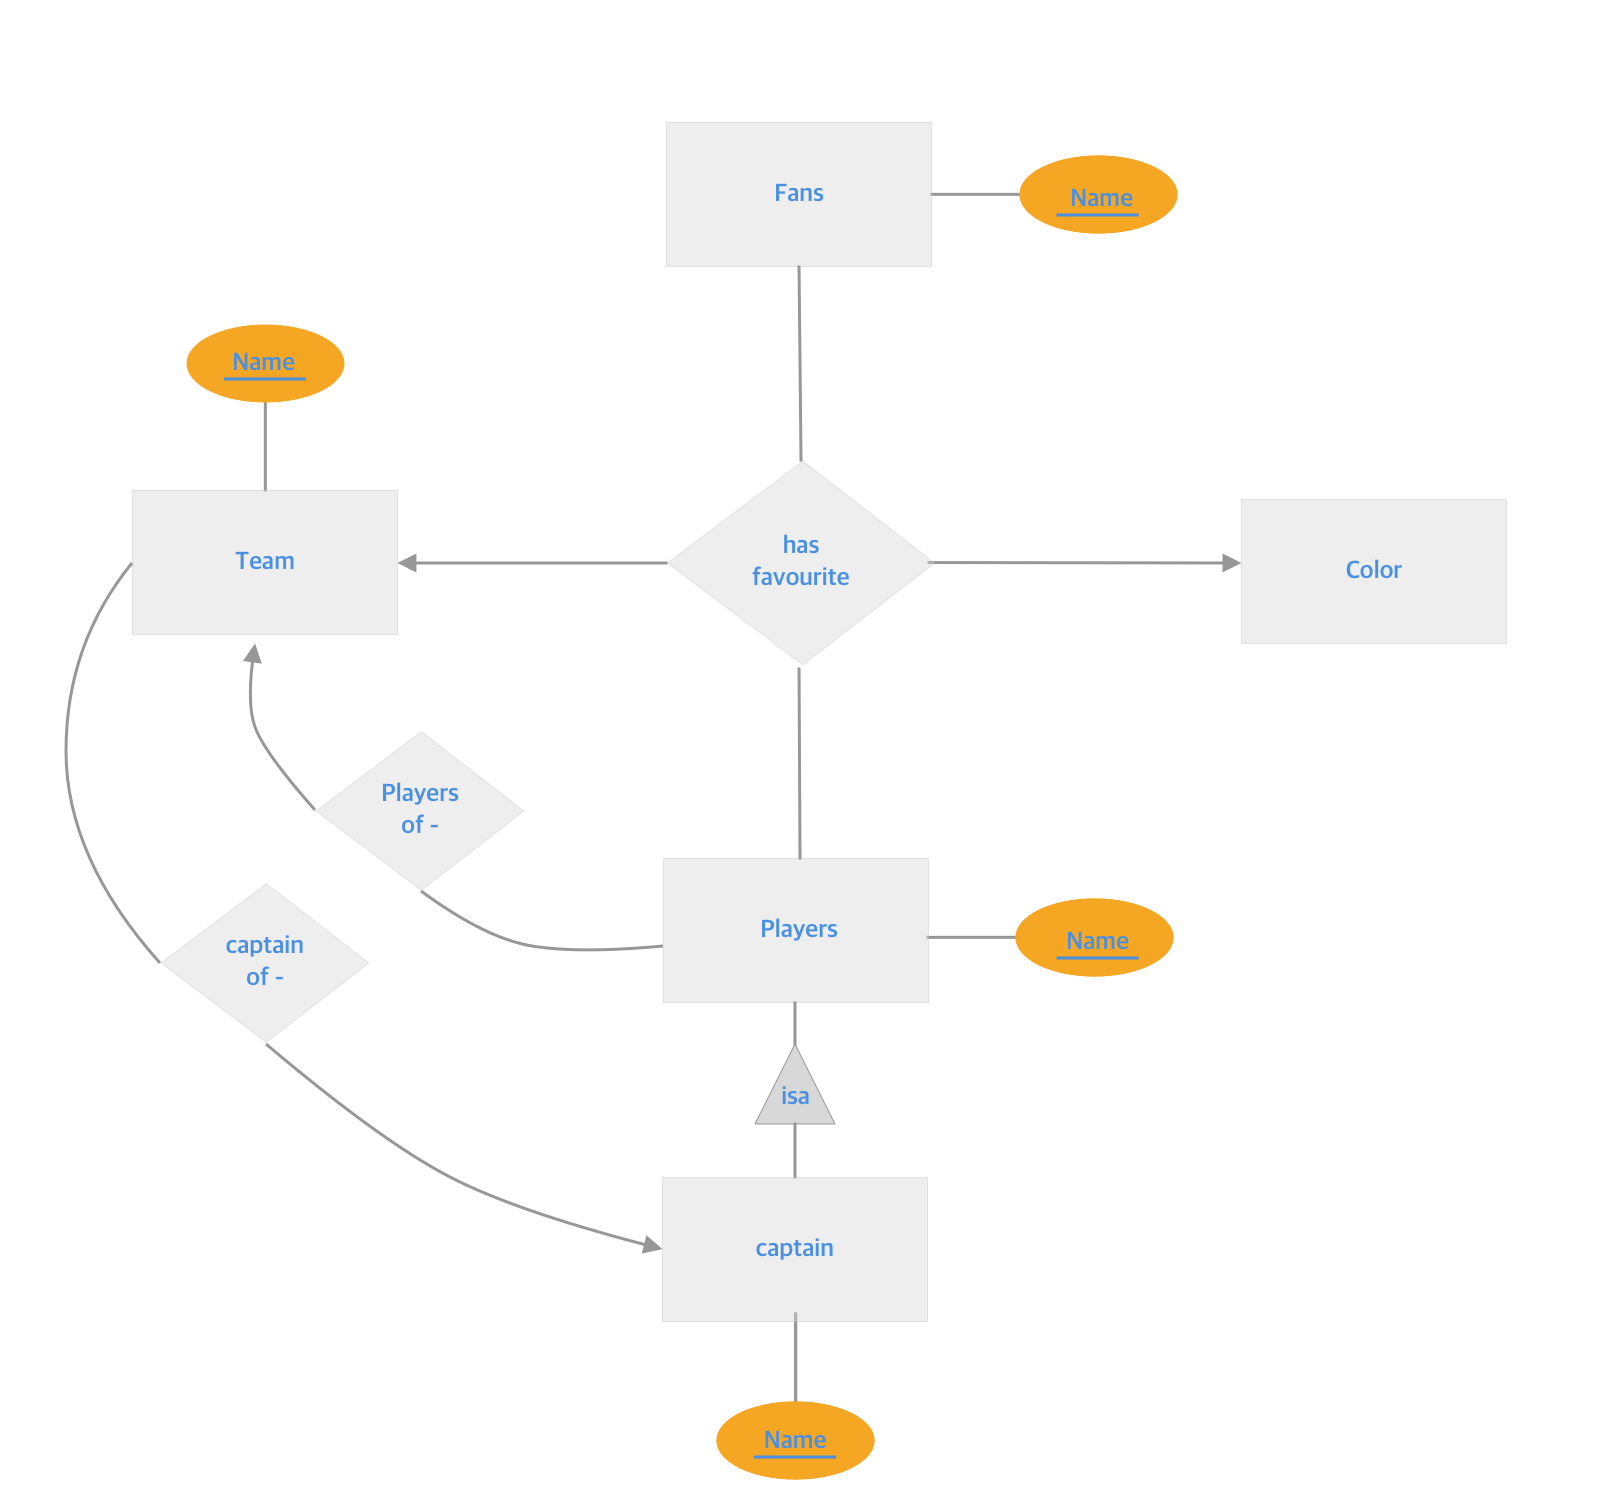
\includegraphics[width=\linewidth]{images/worksheet_15_solution_13.png}
        \end{center}

        \item UML

        \begin{center}
        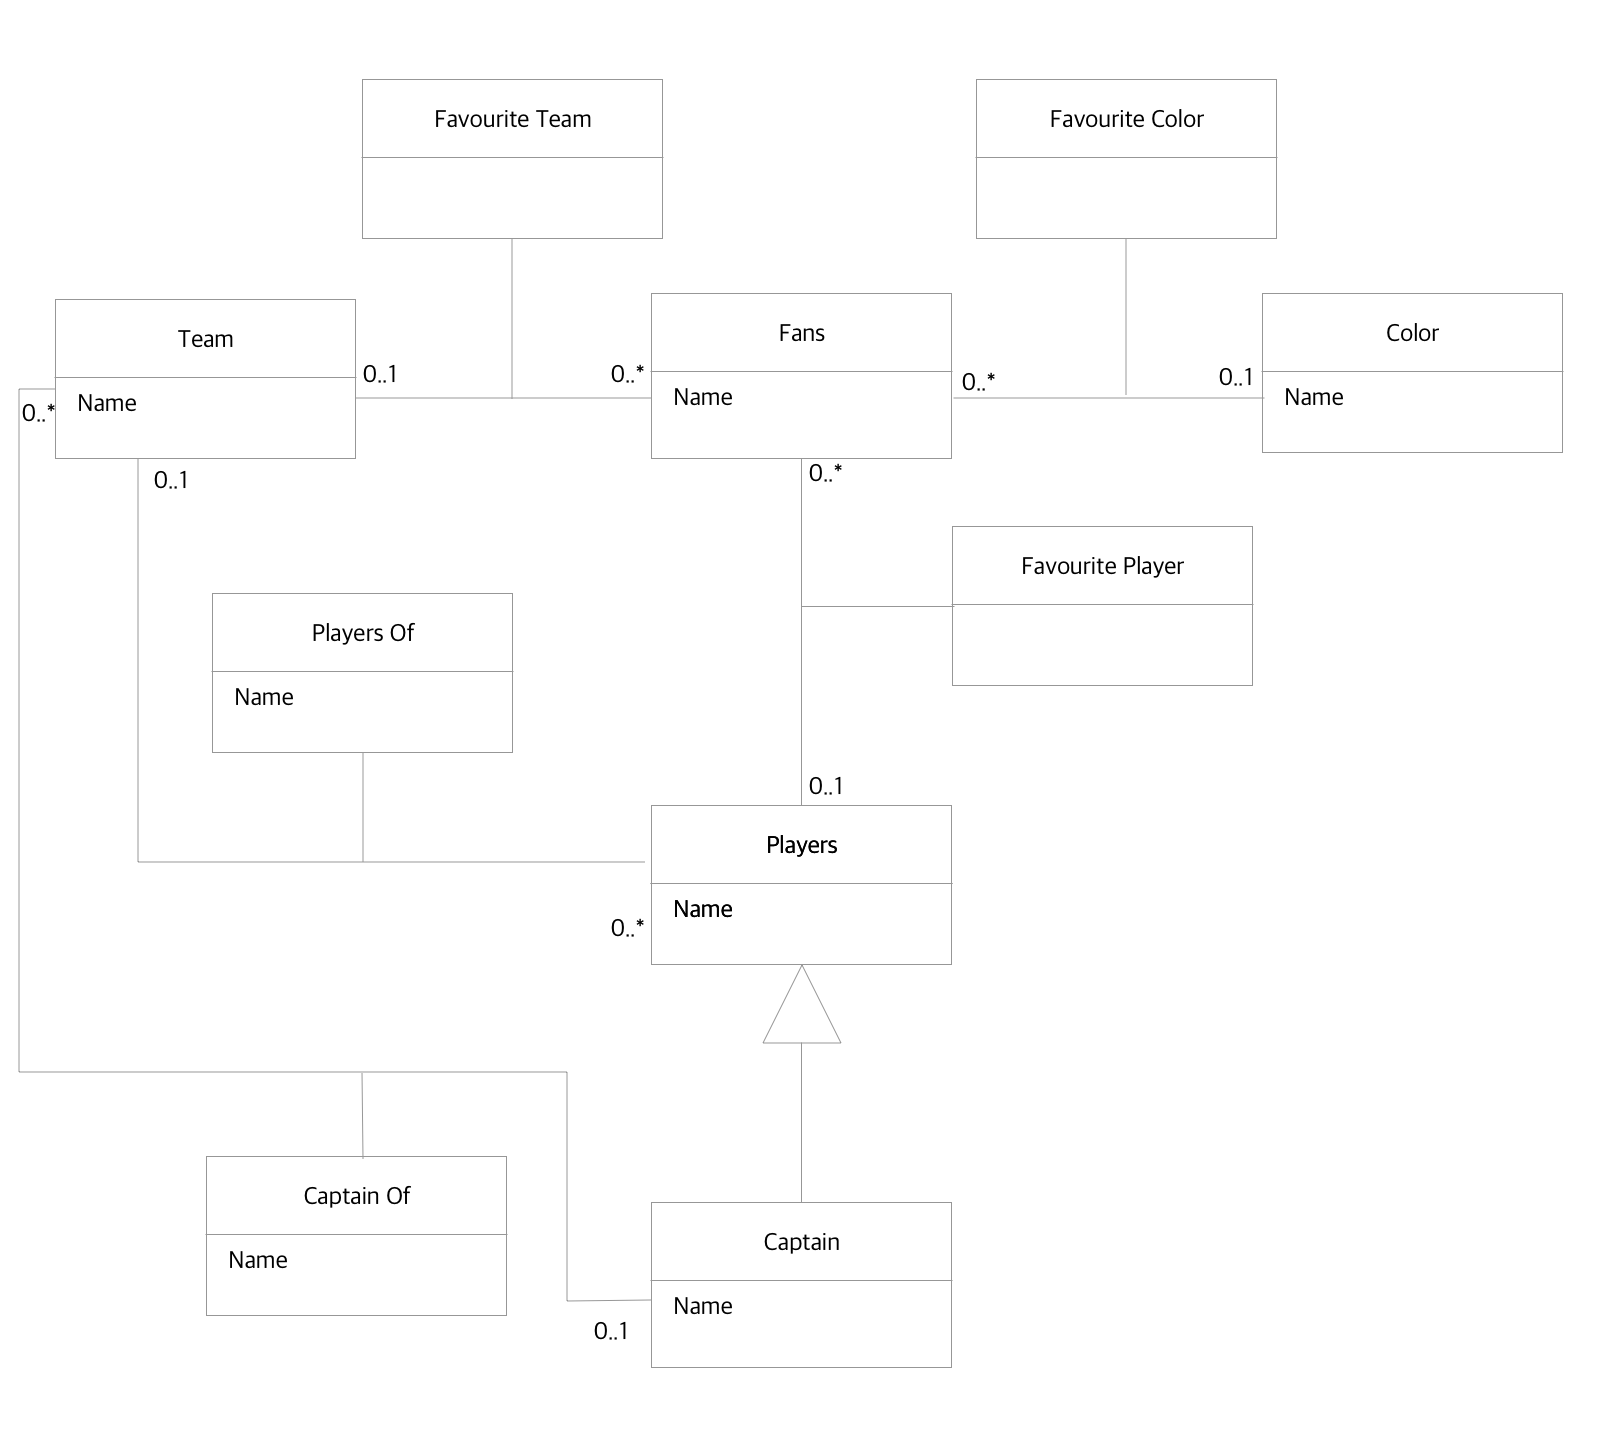
\includegraphics[width=\linewidth]{images/worksheet_15_solution_14.png}
        \end{center}
    \end{itemize}

    \item

    \begin{itemize}
        \item E/R Diagram

        \begin{center}
        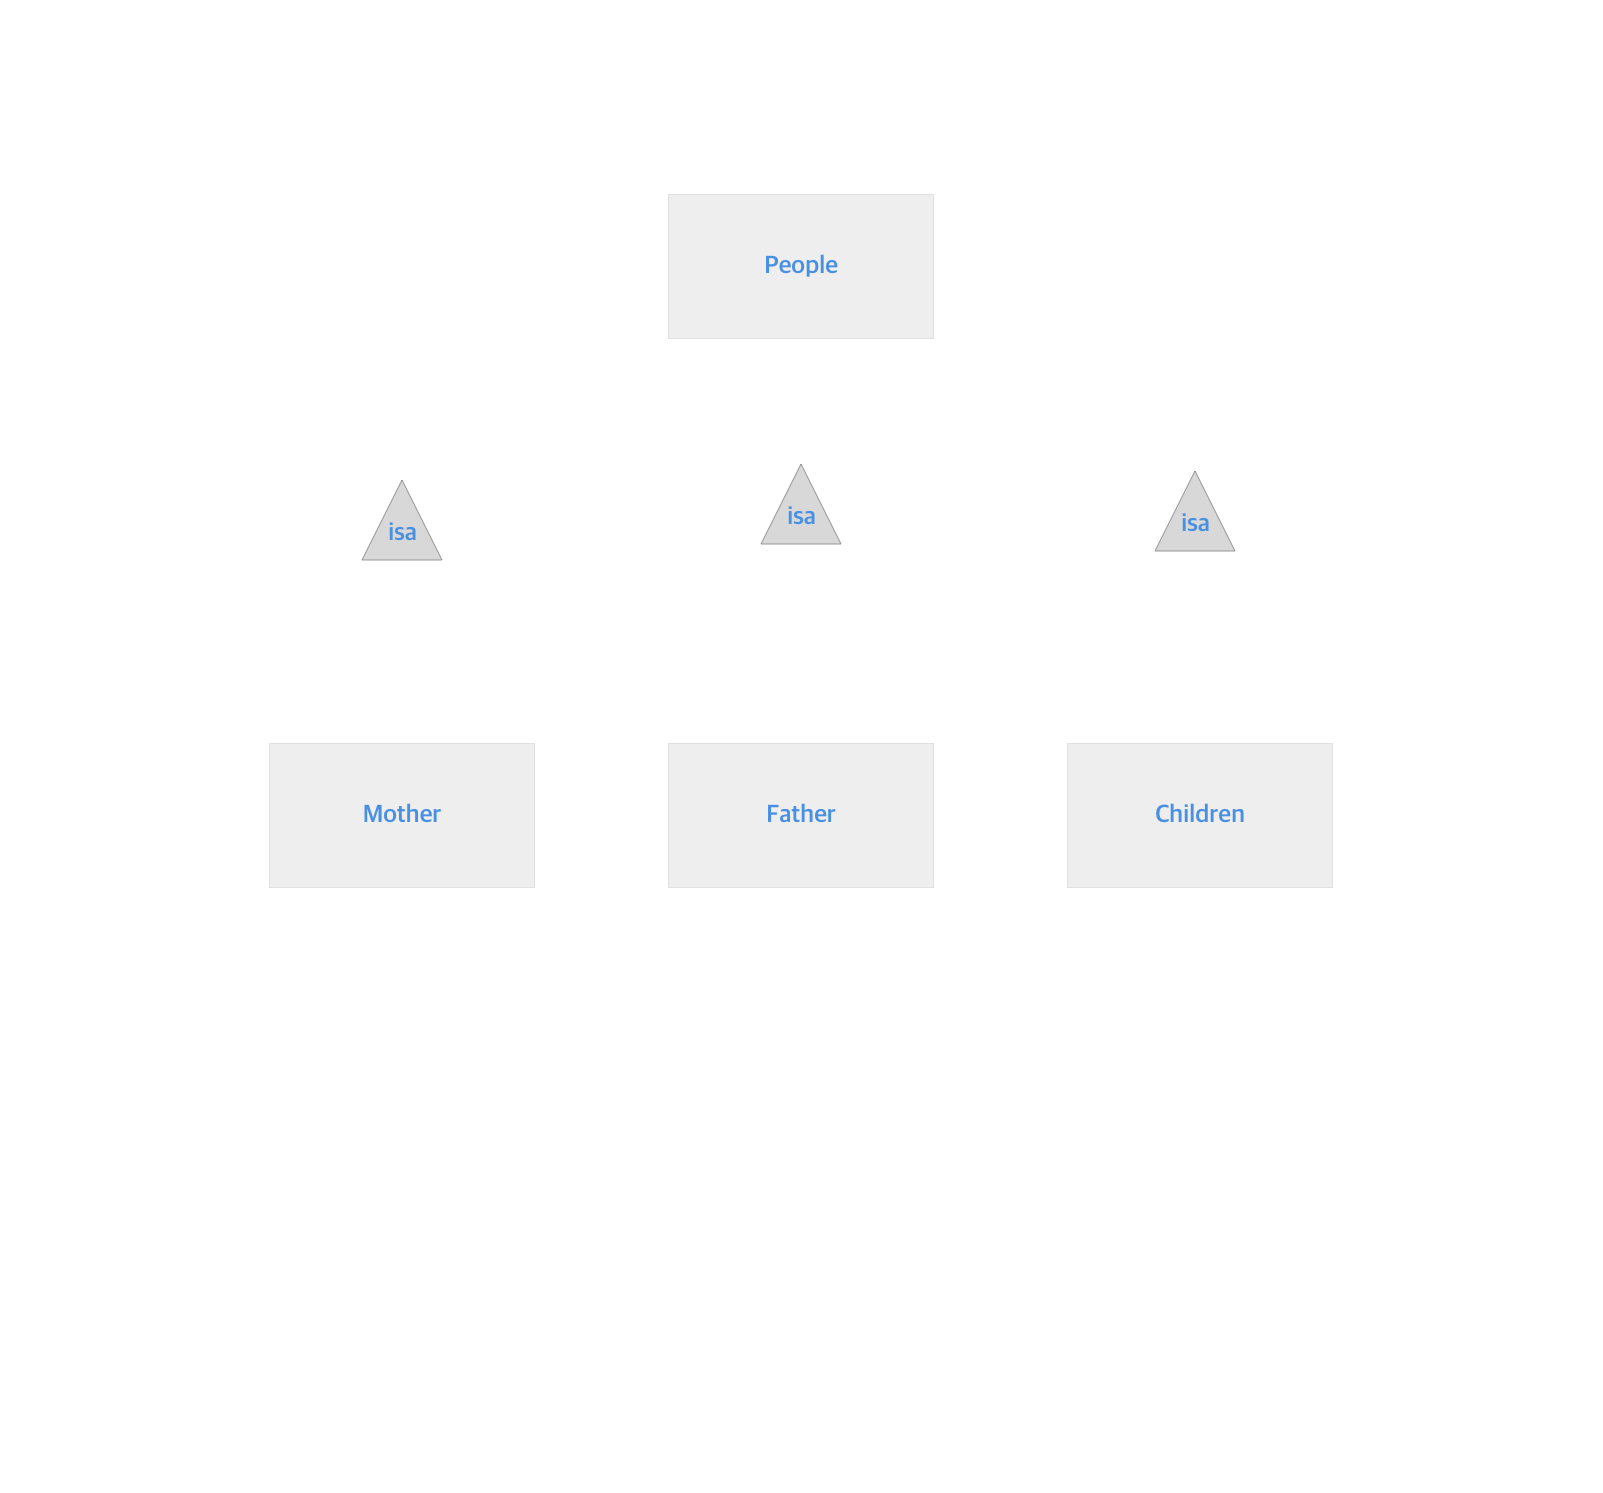
\includegraphics[width=\linewidth]{images/worksheet_15_solution_15.png}
        \end{center}

        \item UML

        \begin{center}
        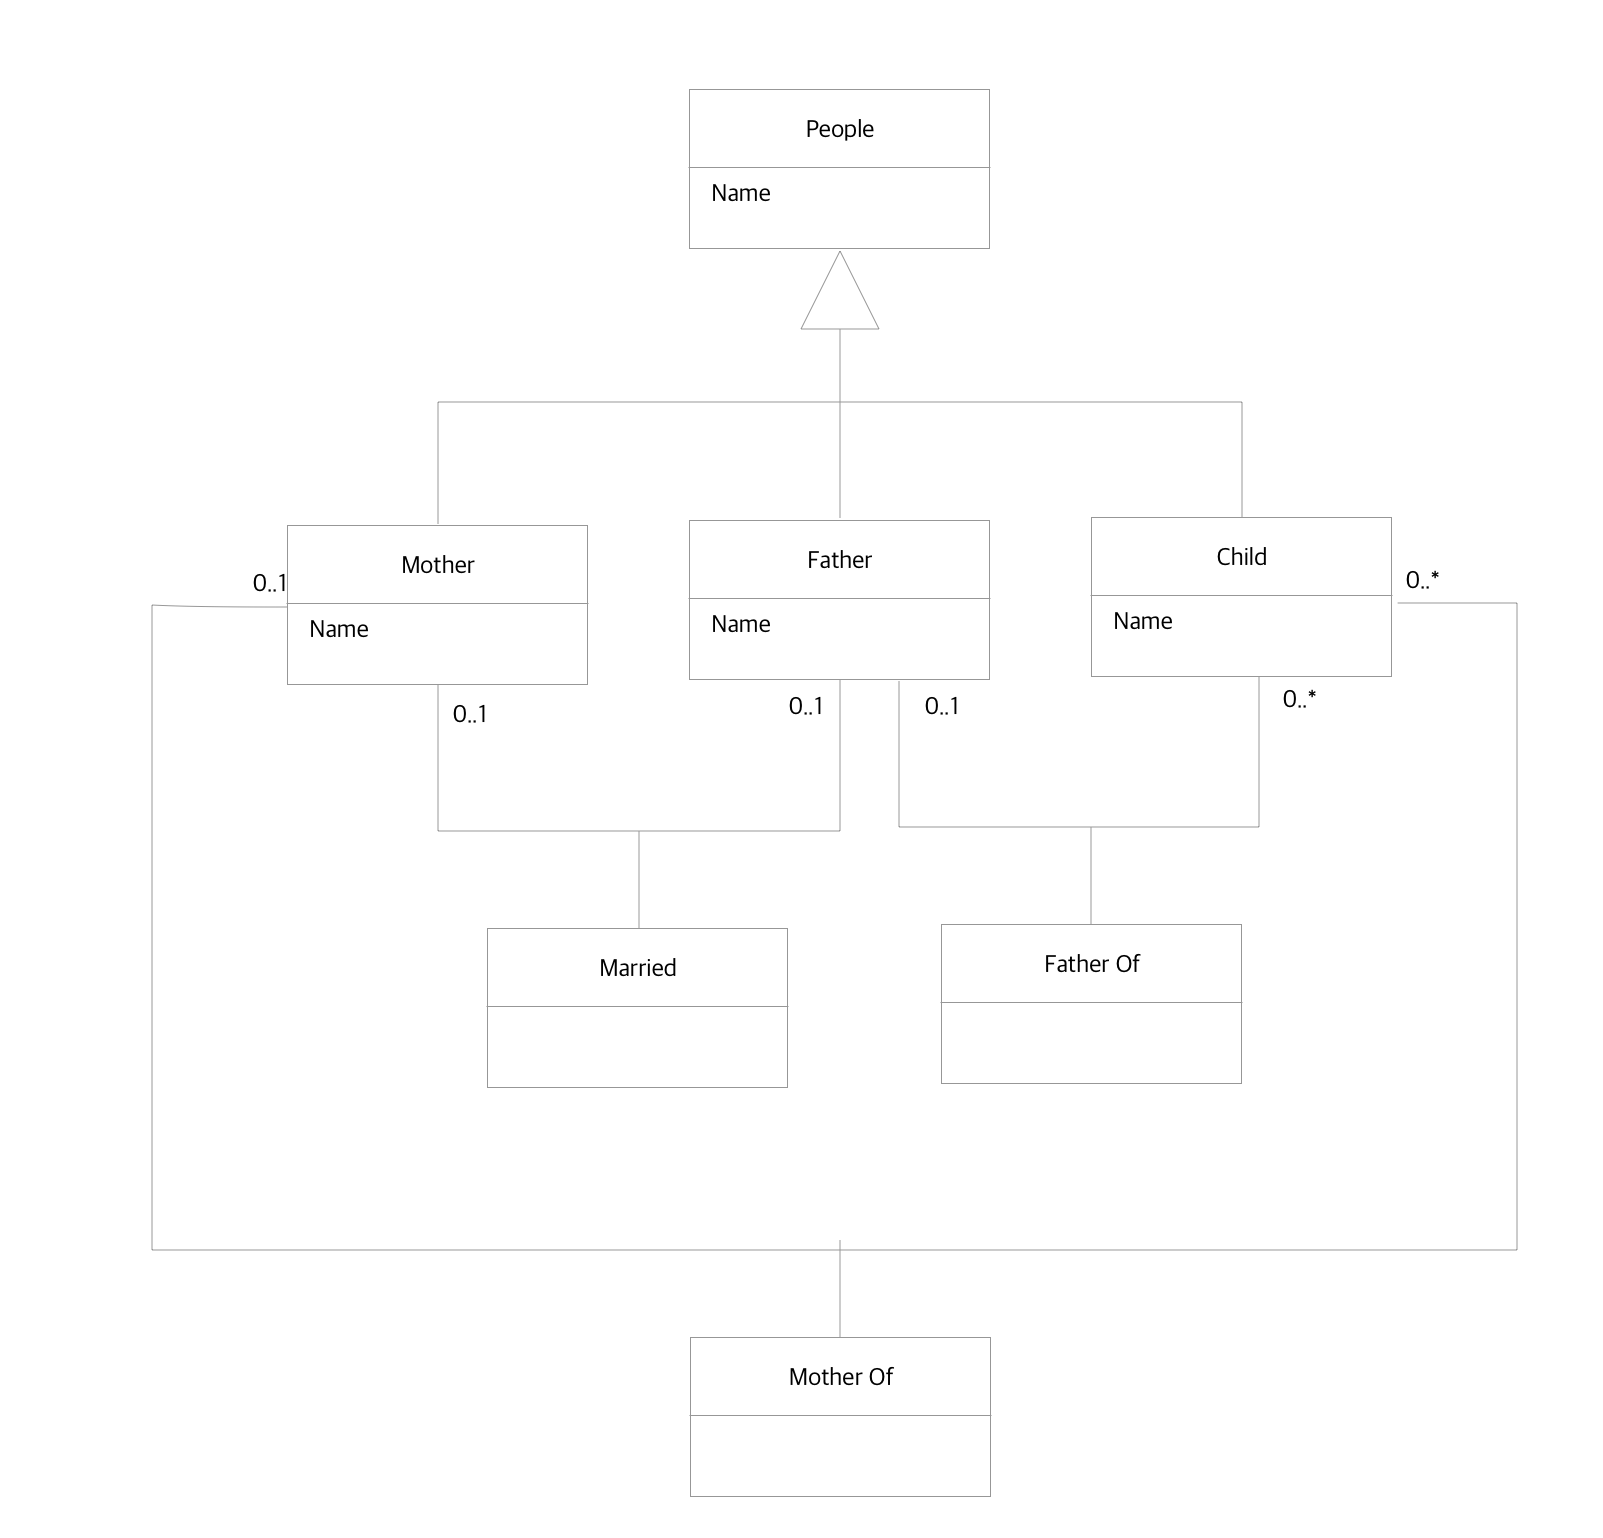
\includegraphics[width=\linewidth]{images/worksheet_15_solution_16.png}
        \end{center}
    \end{itemize}

    \item

    \begin{itemize}
        \item E/R Diagram

        \begin{center}
        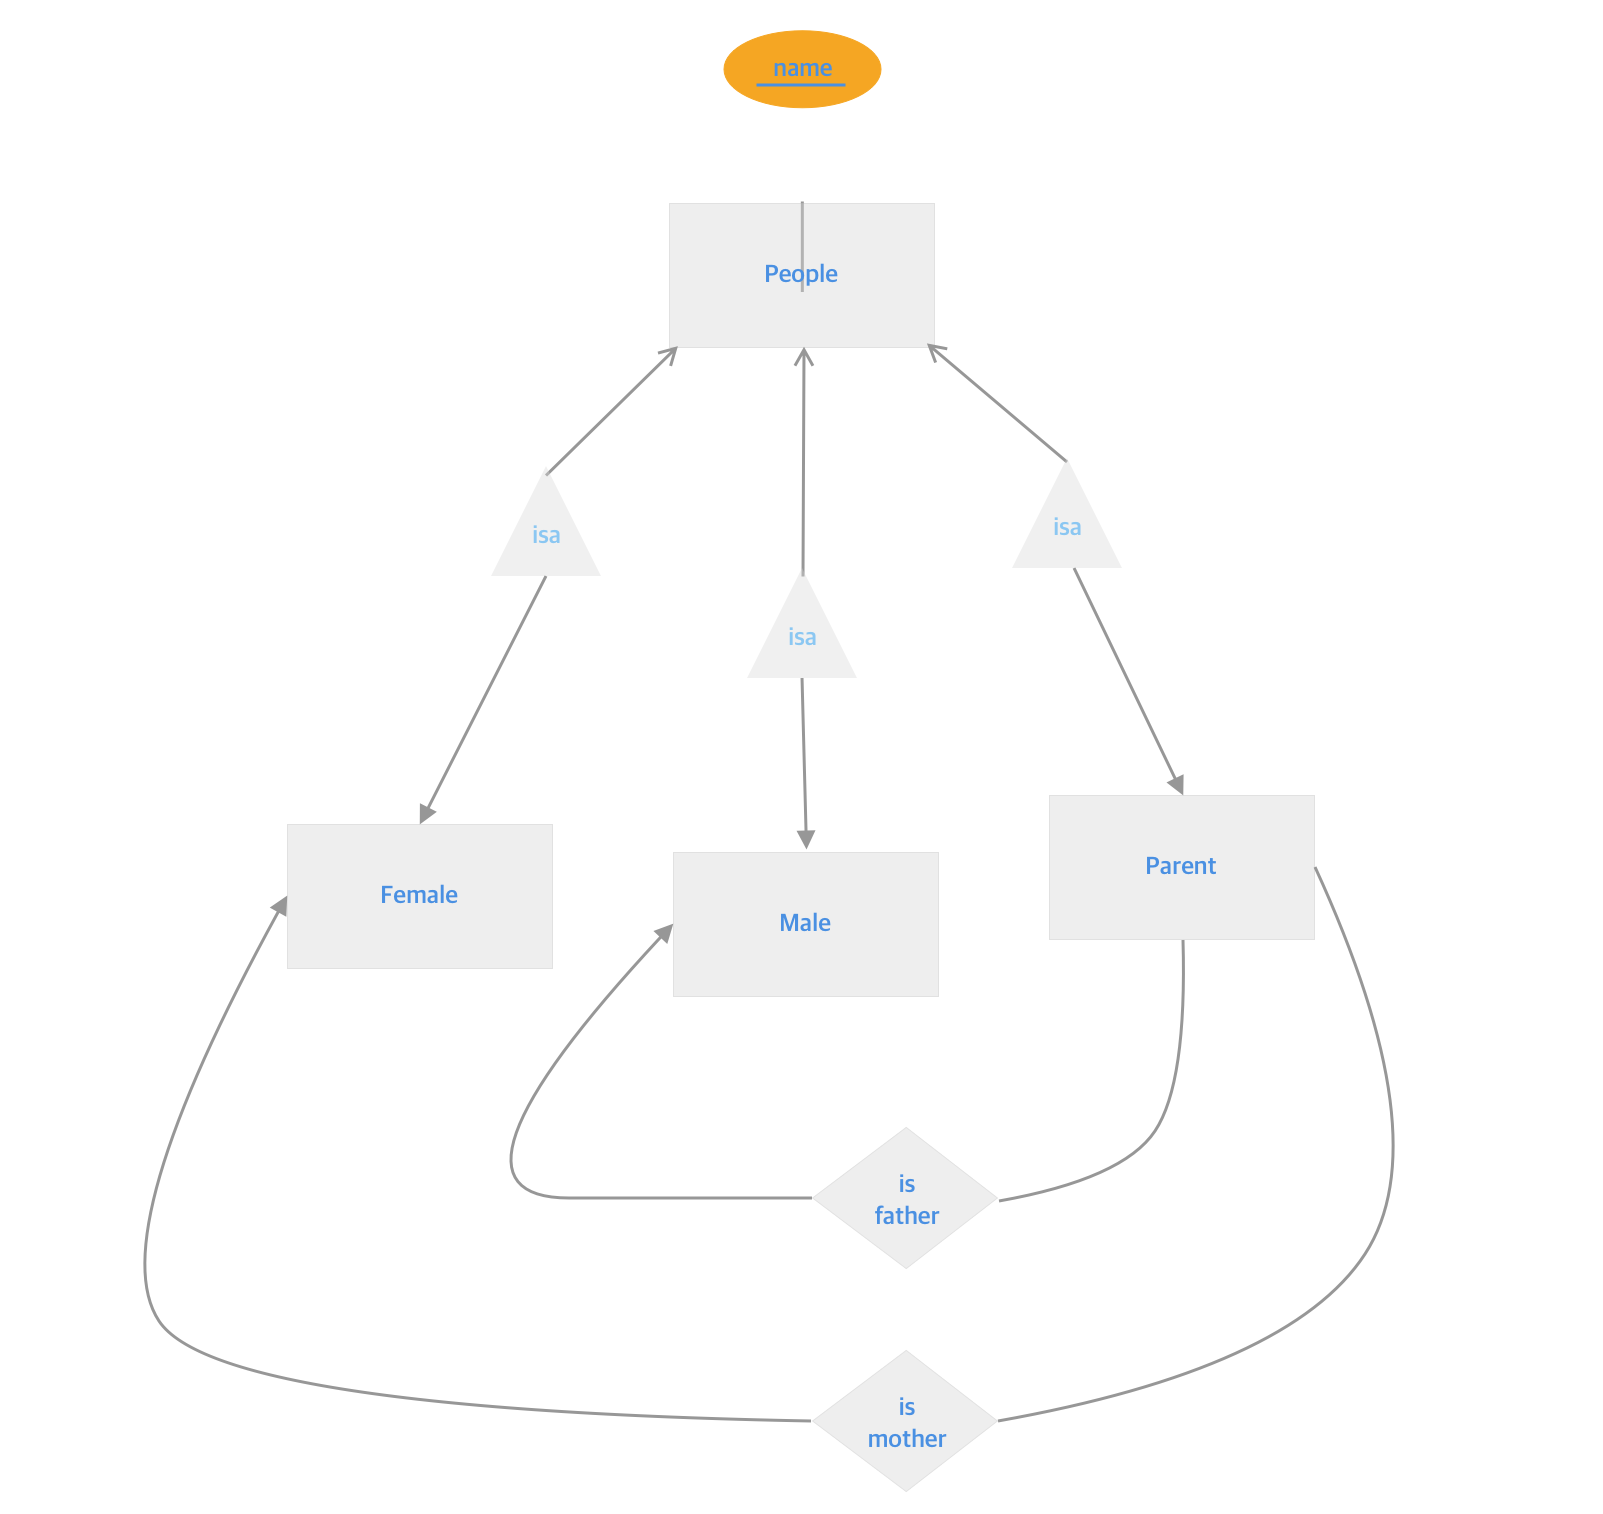
\includegraphics[width=\linewidth]{images/worksheet_15_solution_17.png}
        \end{center}

        \item UML

        \begin{center}
        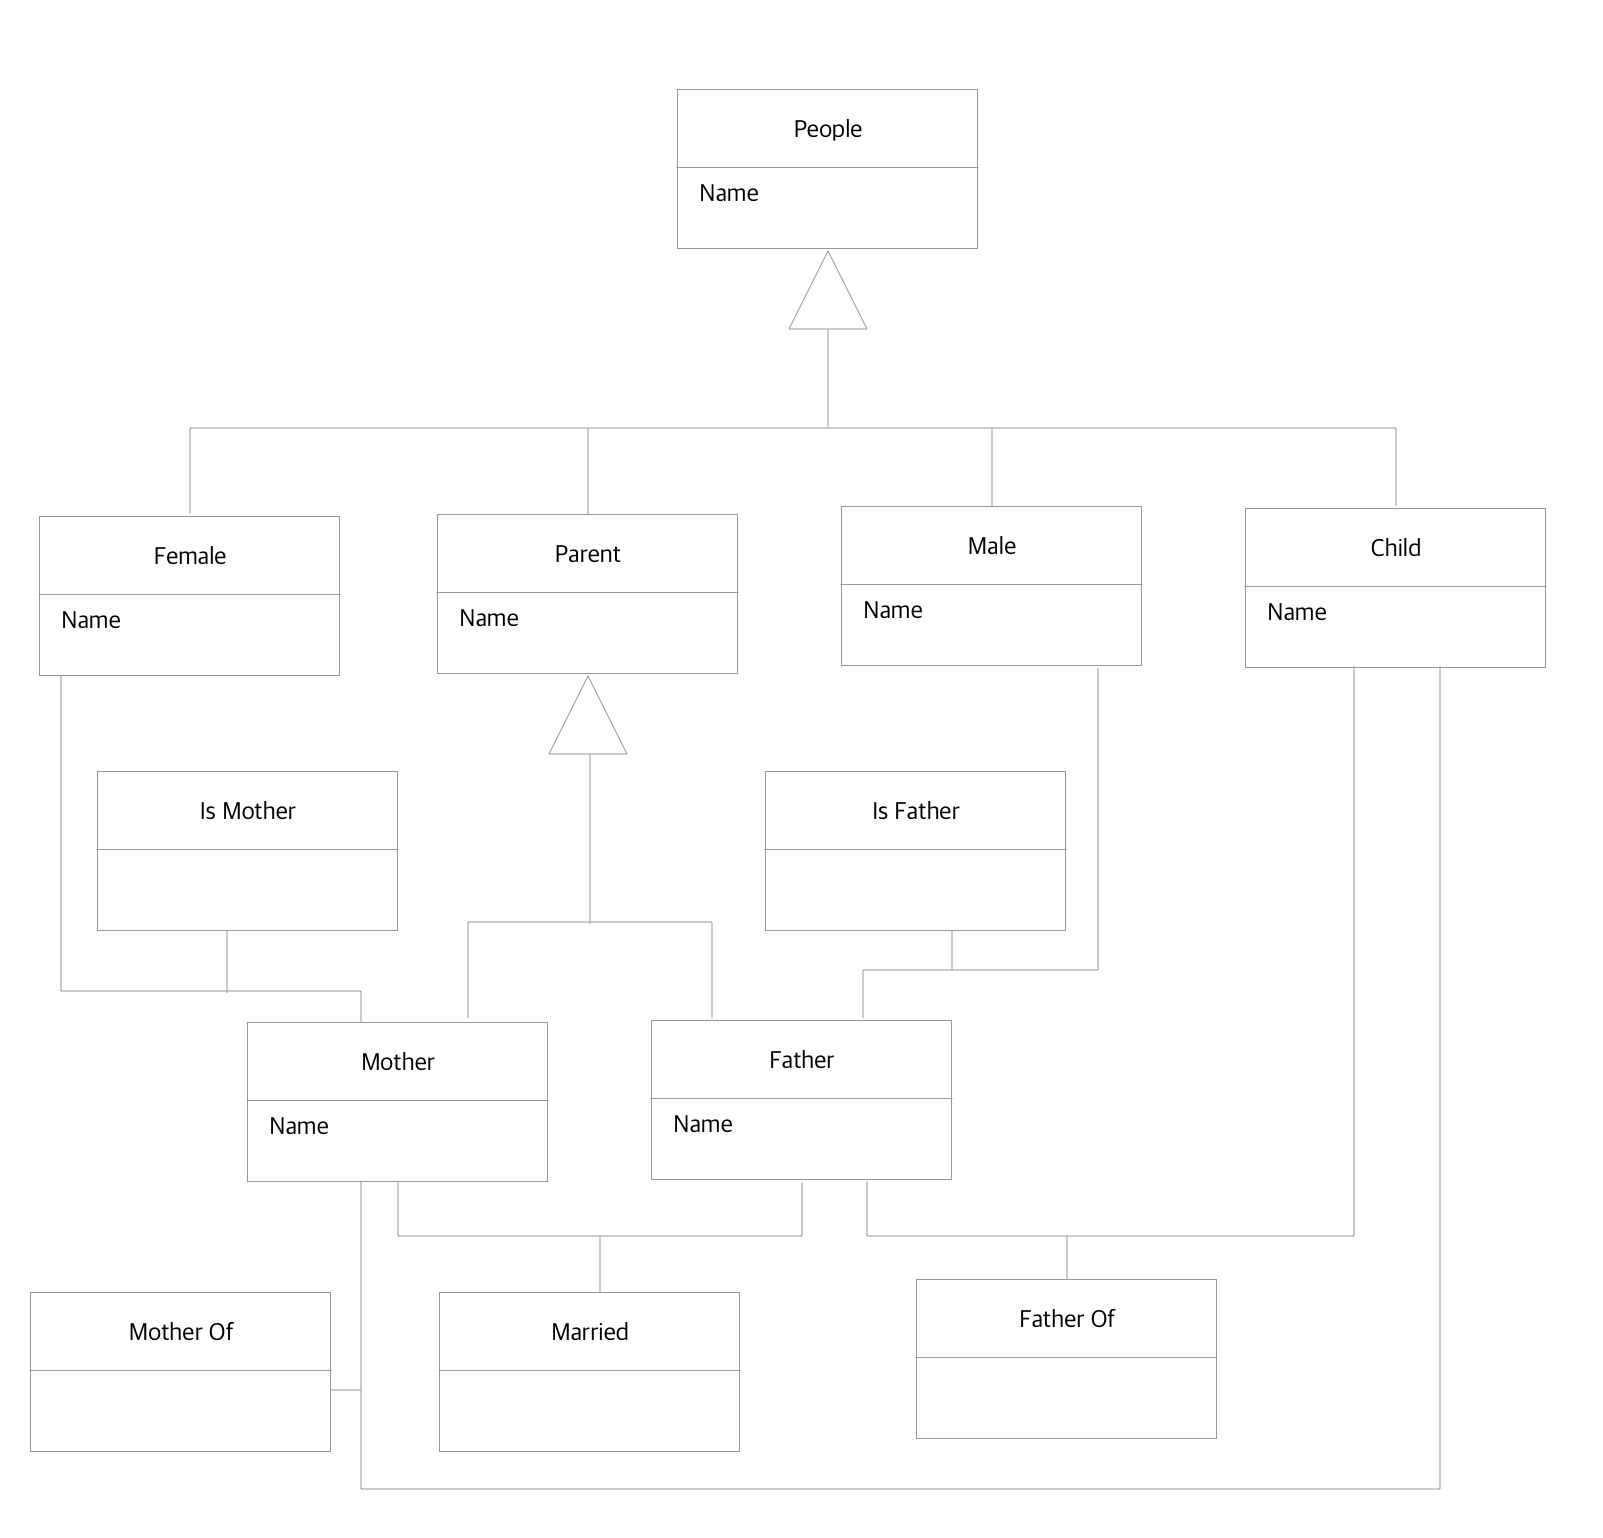
\includegraphics[width=\linewidth]{images/worksheet_15_solution_18.png}
        \end{center}

    \end{itemize}

    \item

    \begin{itemize}
        \item E/R Diagram

        \begin{center}
        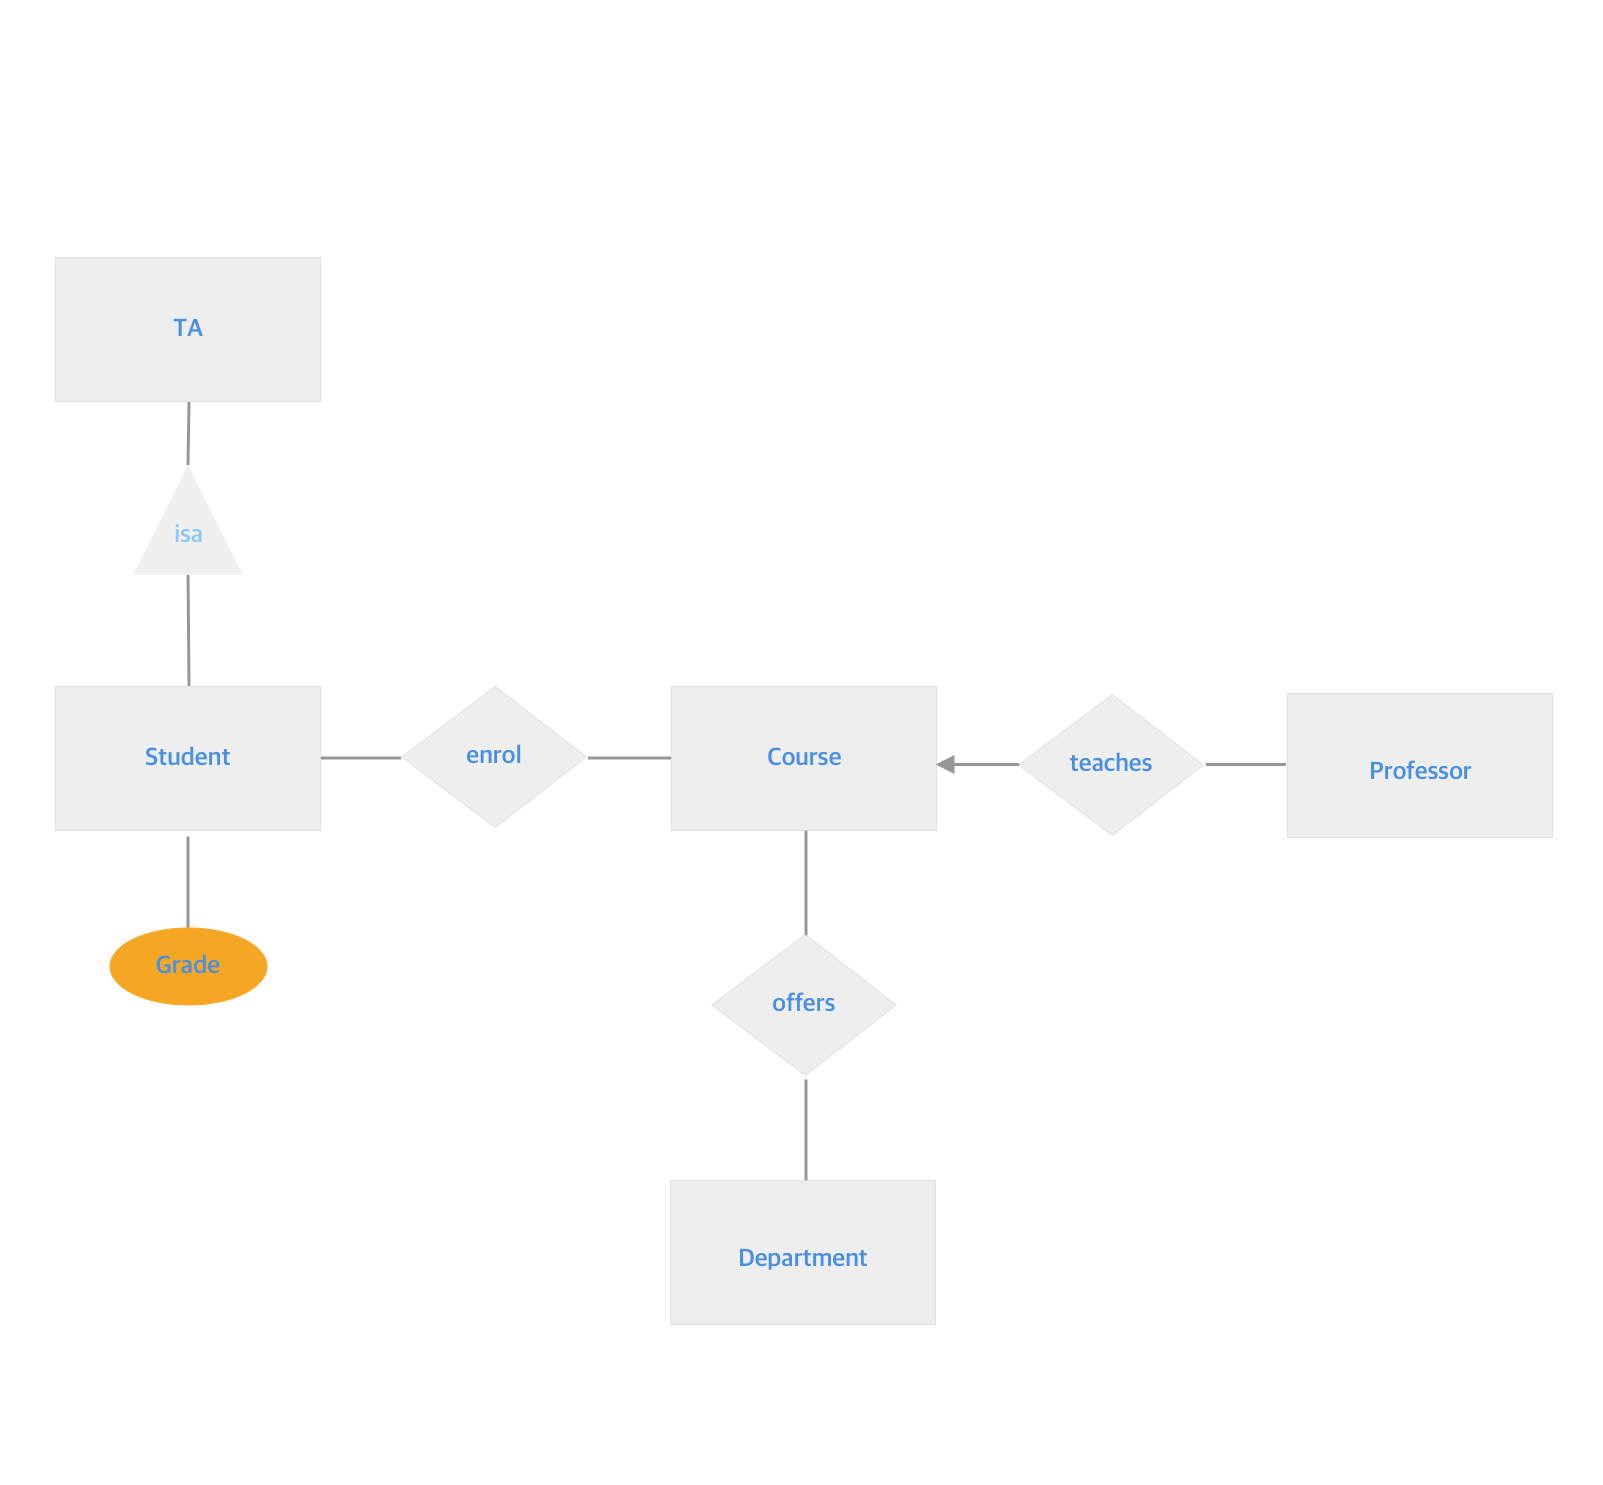
\includegraphics[width=\linewidth]{images/worksheet_15_solution_19.png}
        \end{center}

        \item UML

        \begin{center}
        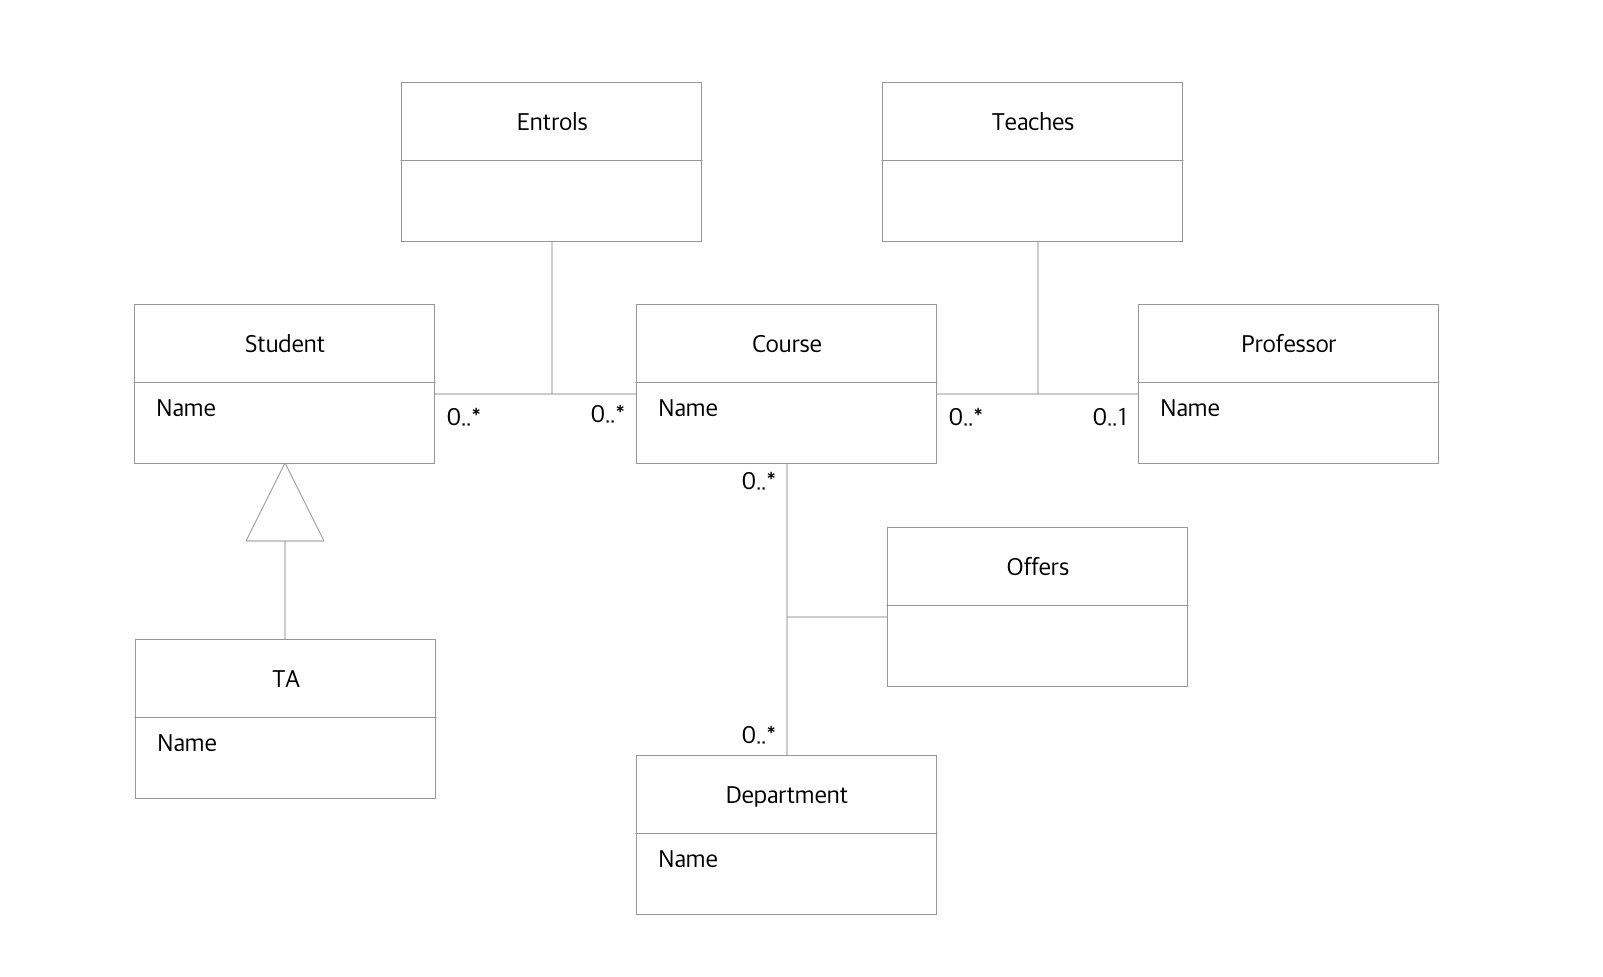
\includegraphics[width=\linewidth]{images/worksheet_15_solution_20.png}
        \end{center}

    \end{itemize}

    \item

    \begin{itemize}
        \item E/R Diagram

        \begin{center}
        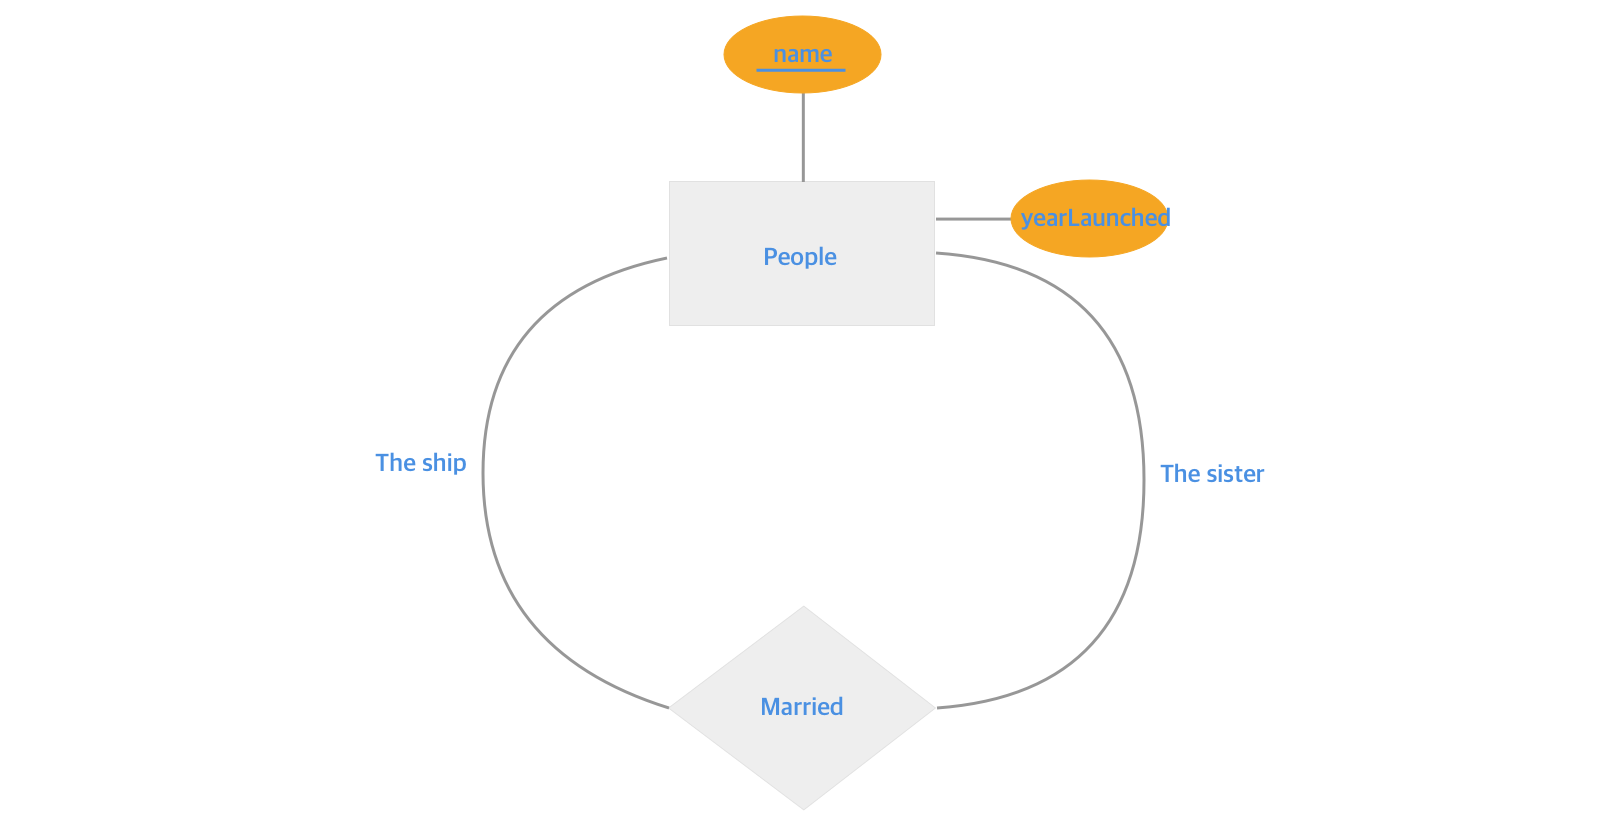
\includegraphics[width=\linewidth]{images/worksheet_15_solution_21.png}
        \end{center}

        \item UML

        \begin{center}
        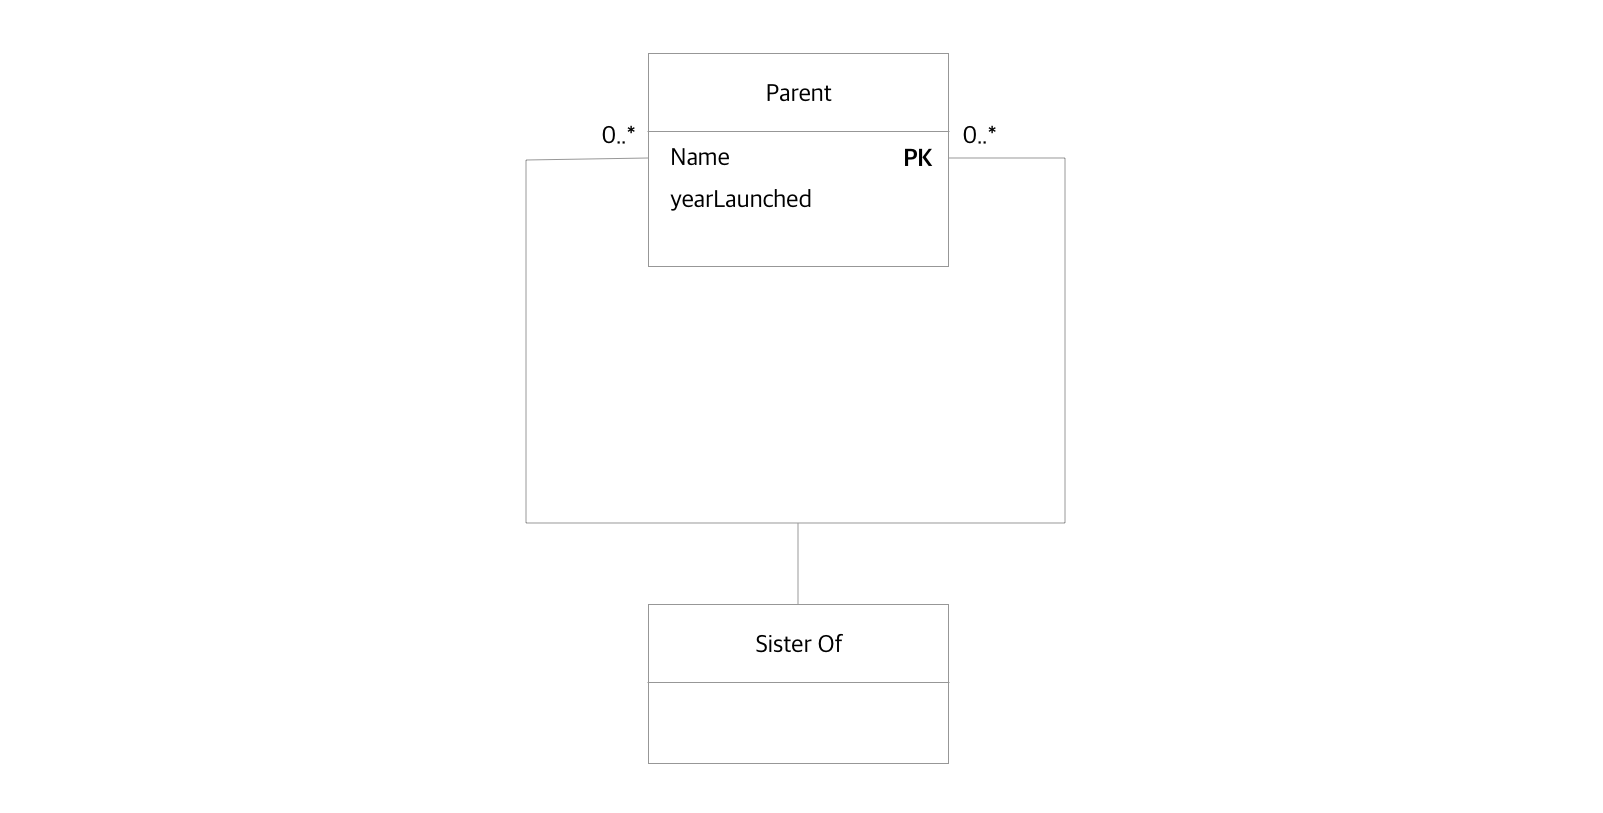
\includegraphics[width=\linewidth]{images/worksheet_15_solution_22.png}
        \end{center}

    \end{itemize}

    \item

    \begin{itemize}

        \item UML

        \begin{center}
        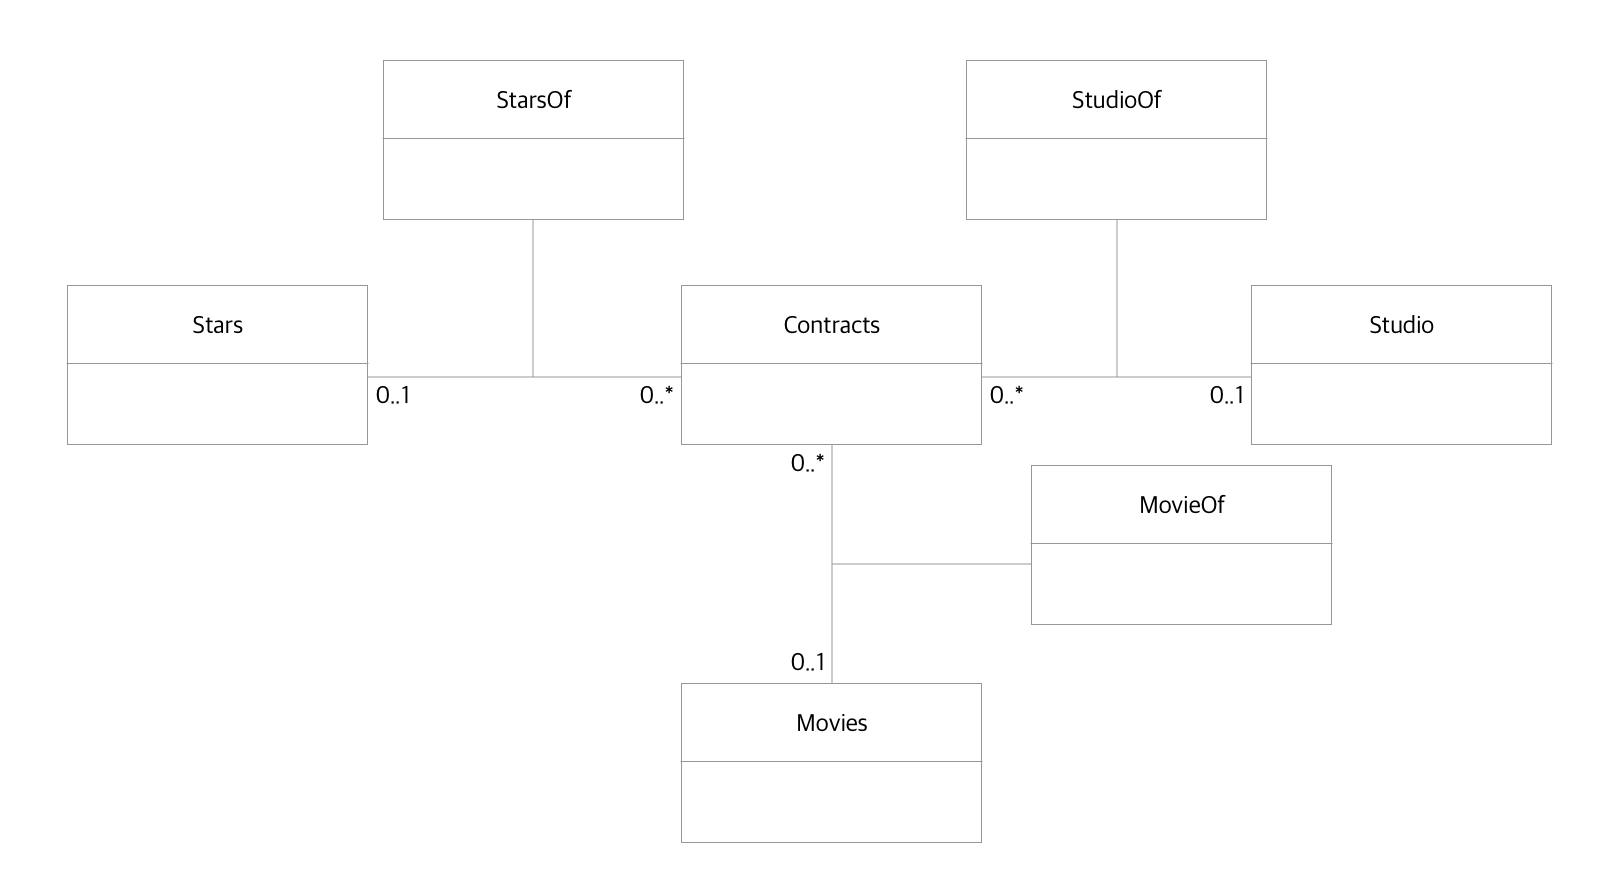
\includegraphics[width=\linewidth]{images/worksheet_15_solution_23.png}
        \end{center}

    \end{itemize}

    \item

    \begin{center}
    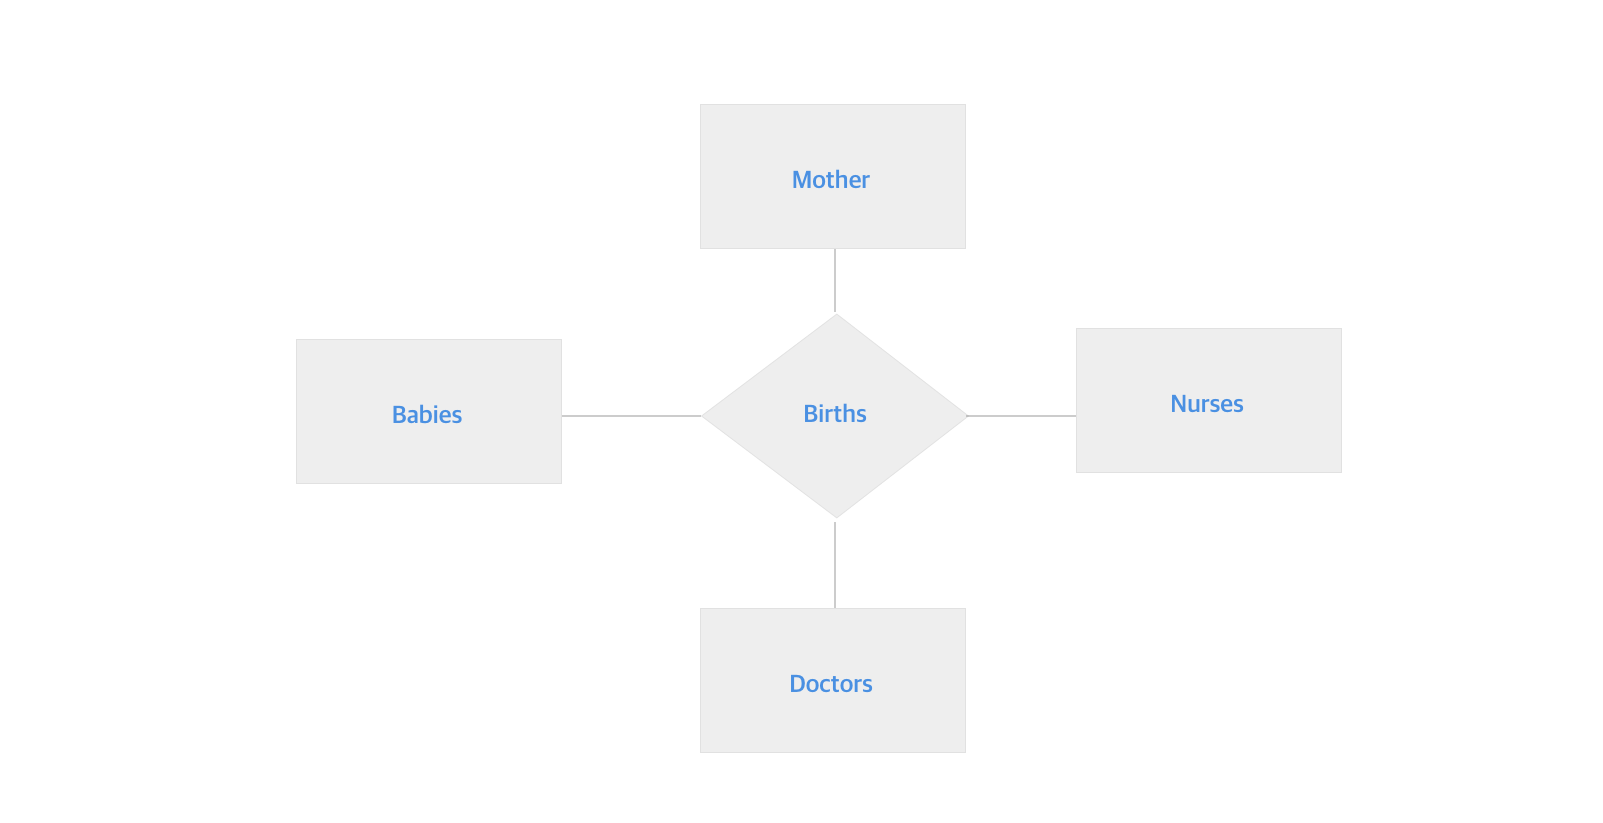
\includegraphics[width=\linewidth]{images/worksheet_15_solution_24.png}
    \end{center}

    \begin{enumerate}[a)]
        \item

        \underline{\textbf{Solution:}}

        \begin{center}
        
\includegraphics[width=\linewidth]{images/worksheet_15_solution_25.png}
        \end{center}
    \end{enumerate}

\end{enumerate}

\end{document}